This work has accomplished two primary goals: defining the intracellular signaling pathway within macrophages that is responsible for inducing angiogenesis during mycobacterial infection (the NFAT pathway) -- a long\hyp{}standing question in the field of tuberculosis pathogenesis -- and setting the stage for future work to simplify and automate common procedures commonly used in the analysis of imaging data relevant to both zebrafish and tissue culture research. This dramatically expands our understanding of the host-pathogen interface in tuberculosis and debunks a widespread assumption, which was that hypoxia signaling is primarily responsible for the angiogenic response surrounding the granuloma. Instead, there is a discrete and specific immunological pathway that drives the expression of VEGFA to induce angiogenesis that seems to be functionally independent of hypoxia \textit{sensu stricto}\footnote{This argument is supported by the fact that the larval zebrafish is oxygen perfuse, so hypoxia was clearly not the driving trigger in this context. Hypoxia may, however, synergize or otherwise interact with these immunological pathways within more mature granulomas in the adult, a question that will be addressed further in \autoref{hypoxia}.}. This sets the stage for the subversion of other assumptive dogmas within the field, including what functional roles angiogenesis contributes to the growth or survival of mycobacteria. At the conclusion of the present work, many new questions have been generated while others remain unanswered and these offer fertile ground for new discoveries in the field of tuberculosis pathogenesis and host immunity. 

Some of these lingering questions will be addressed in the coming weeks and months while others will stretch over the course of many years or decades as we delve into deeper and more sophisticated understandings of the fundamental processes governing the nature of the angiogenic response to tuberculosis infection and how and when this can be a fruitful target for therapeutic intervention. This leaves a set of important questions (\autoref{figure:lingeringquestions}) pertinent to model development, nuanced understanding of the biology of NFAT within (granuloma) macrophages, the intersections between this pathway and other, known pathways involved in angiogenic responses, and the future of imaging analysis in the context of ever\hyp{}growing computational power. 

\begin{itemize}
\item What is the TDM receptor in zebrafish and do they have an as\hyp{}yet unannotated MINCLE homolog functionally equivalent to the human gene? 
\item How or why is NFATC2 special and is it sufficient to induce VEGFA or are there other factors also required for VEGFA expression? 
\item How does the NFAT pathway alter other aspects of macrophage behavior potentially relevant to tuberculosis biology and does this pathway intersect with HIF\hyp{}1$\upalpha$ signaling? For instance, does this interface with dimensions of immunometabolism potentially mediated by hypoxia or other alterations in macrophage physiology?
\item Do mycobacteria have other mechanisms for manipulating host vasculature and, if so, what are they and how can that enhance our overall understanding of the contributions of the vasculature to tuberculosis pathogenesis? 
\item Are our findings on the nature of NFATC2 in inducing tuberculous angiogenesis relevant to other disease contexts where VEGF signaling plays an important role? 
\item Could NFAT offer a meaningful mechanism for inhibiting angiogenesis in the context of disease as a host\hyp{}directed therapy?
\end{itemize}

These questions, among many others, are the subject of this concluding chapter and are summarized in \autoref{figure:lingeringquestions}; it is hoped that a comprehensive presentation of these questions will stimulate future generations to pursue answers and that these will further inform our understanding of the pathogenesis of tuberculosis toward the goal of eradicating this contagion.

\begin{figure}
\centering
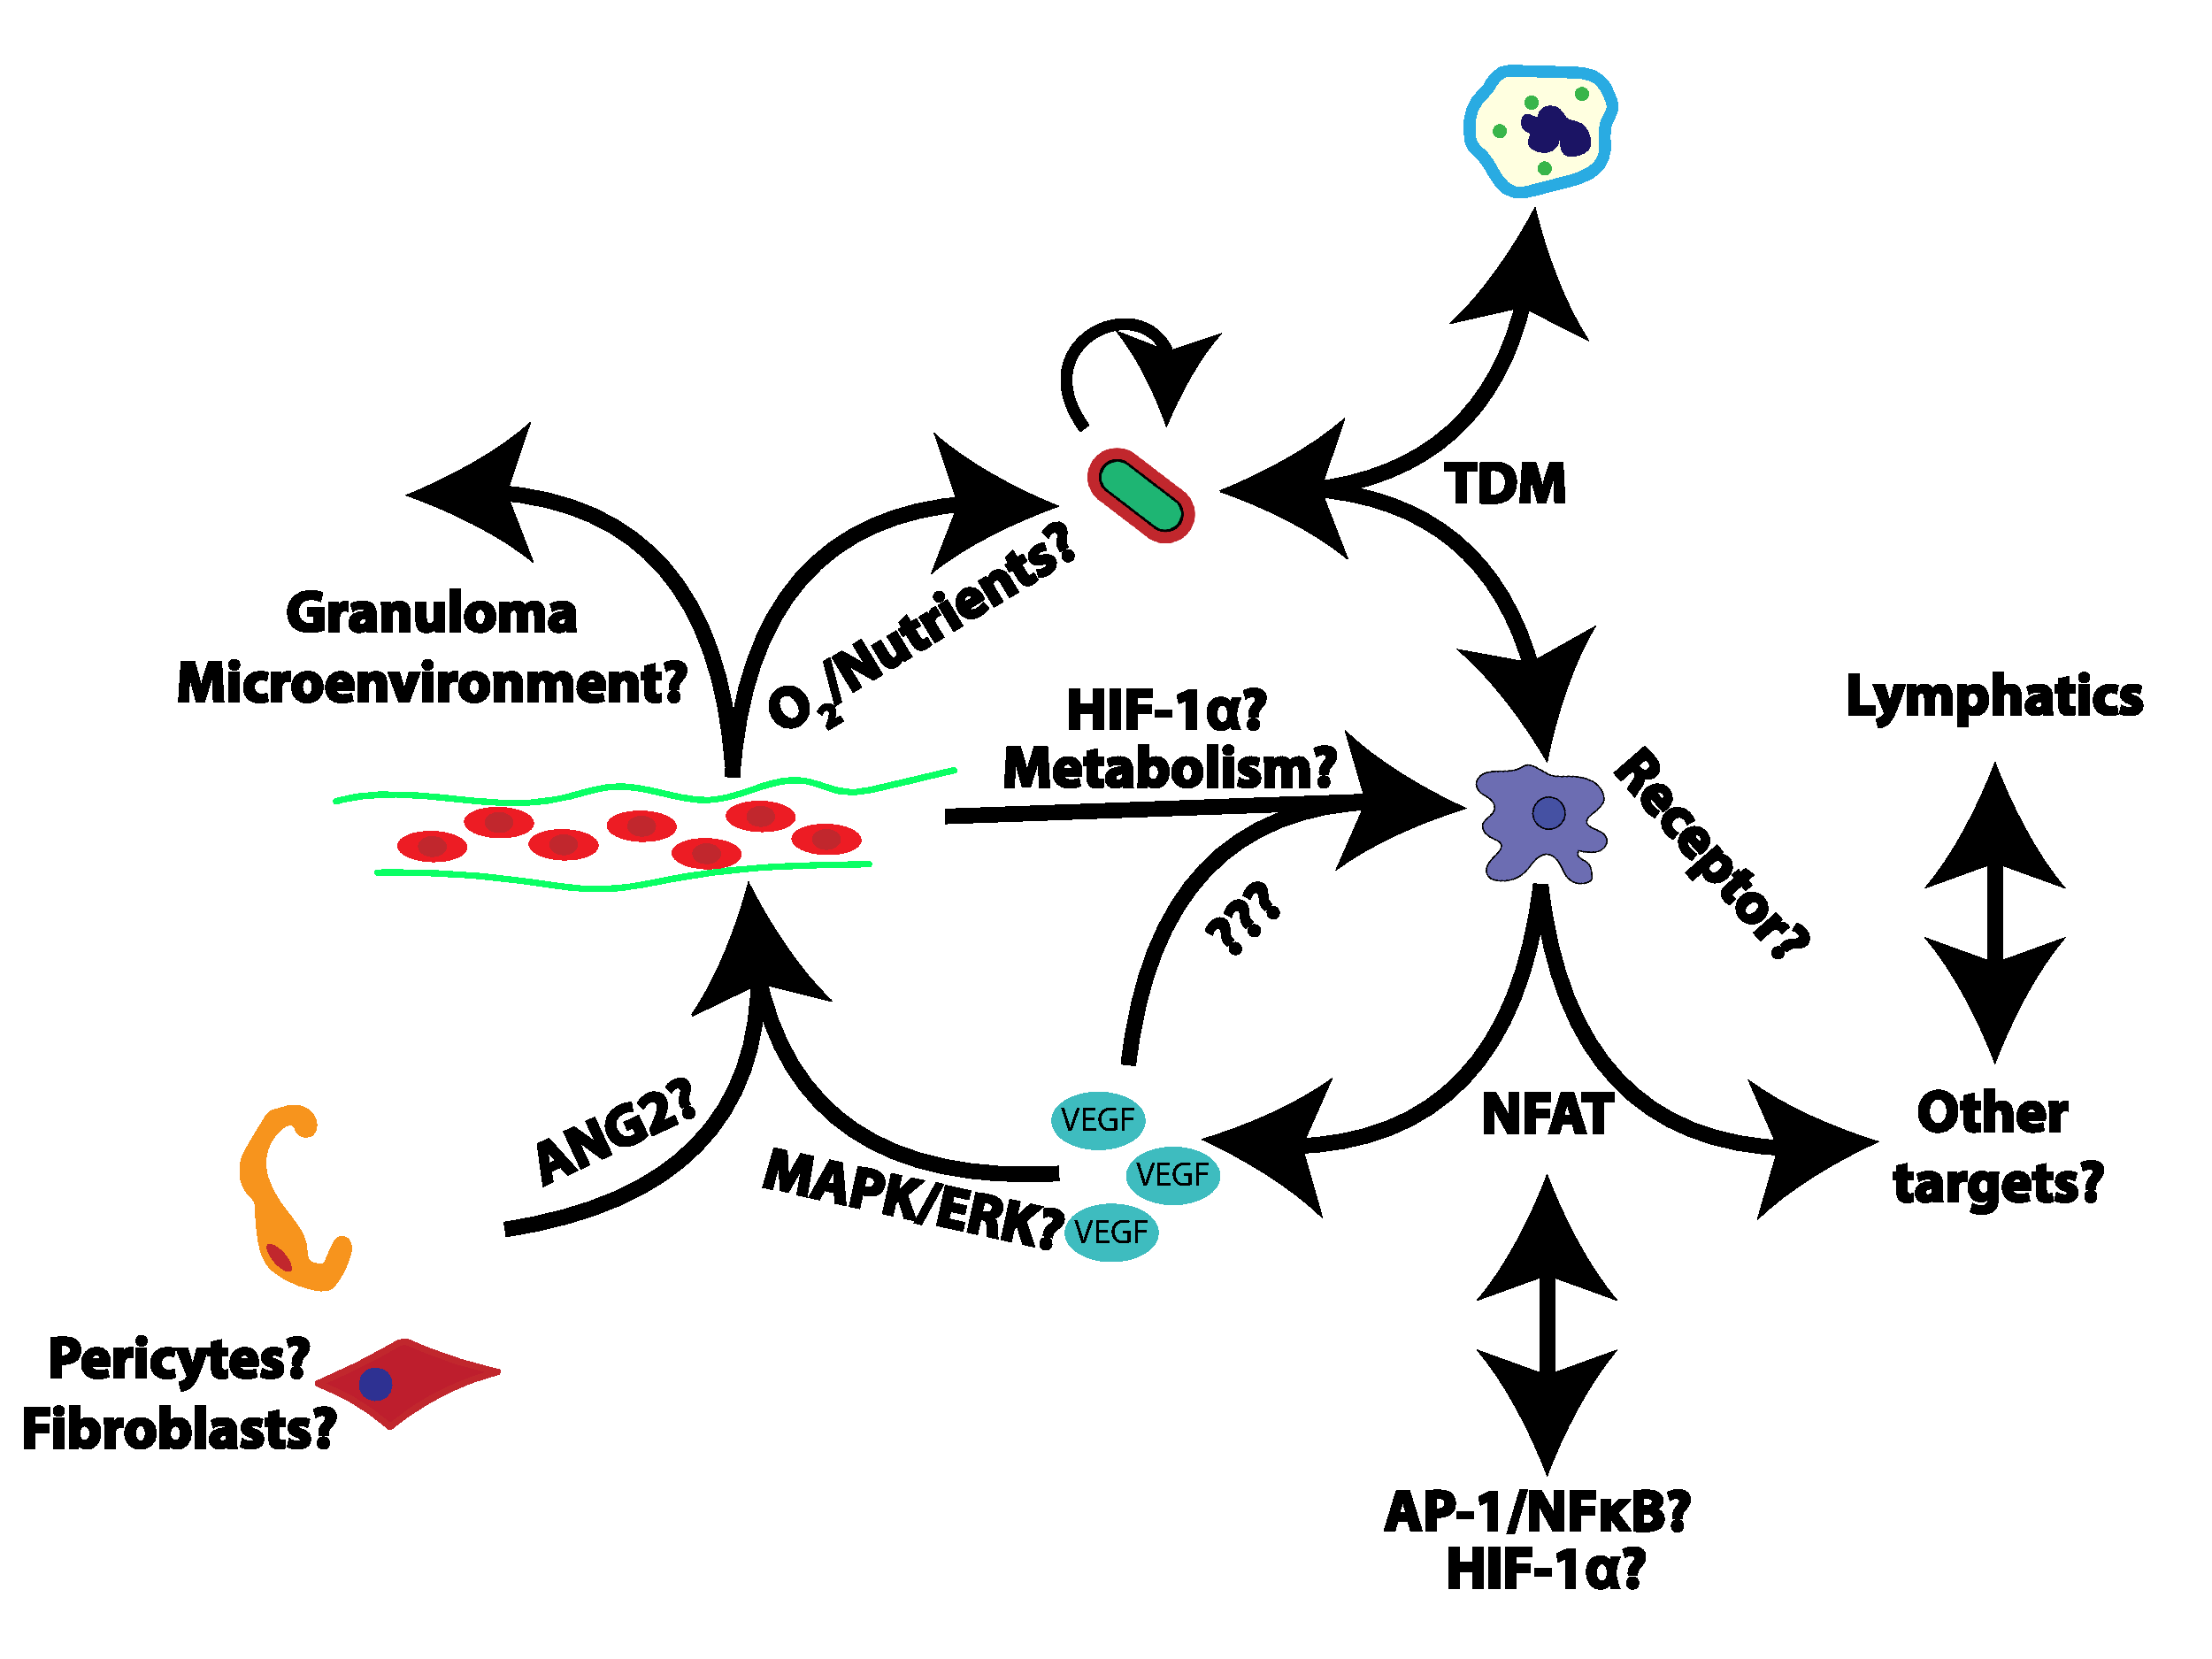
\includegraphics[width=\textwidth]{images/lingeringquestions.pdf}
\caption{A graphical representation of the major findings and questions from this work. While we have now added a critical piece of the equation, there are many questions remaining and many directions for this project to go that effectively interrogate each of the different players, from the bacteria to macrophages to the endothelium and interesting aspects of the interactions between them which will be outlined in the coming sections.}
% Provide a label so we can cross\hyp{}reference it from the tex
\label{figure:lingeringquestions}
\end{figure}

\section{The Zebrafish MINCLE}\label{zfmincle}

As discussed in \autoref{tdmreceptor}, data from human cell culture and mice has implicated MCL and MINCLE as the primary C\hyp{}type lectin receptors for TDM, which induces a variety of downstream responses, seemingly including the upregulation of VEGF and downstream angiogenesis (see \autoref{chap3}). However, the precise identity of the homolog of MCL or MINCLE in the zebrafish remains unknown, making it difficult to precisely model these process or make one\hyp{}to\hyp{}one comparisons between humans and the zebrafish. In human, these two proteins arose from a tandem duplication and inversion at an unknown point in evolutionary history, although the two are ubiquitous across reptiles, birds, and mammals \citep{Miyake2013, Richardson2014}. Given the strong, bidirectional selective pressure on both host and pathogen to modulate host PRR activity, these divergences are expected even between closely related species \citep{Rambaruth2015}. This diversification is especially notable among CLRs: mice have no fewer than eight putative DC\hyp{}SIGN homologs and a great deal of work had to be done to narrow down the functional ones in order to model human disease \citep{GarciaVallejo2013}; on the other hand, the bovine homolog of MINCLE was readily identifiable but had diverged in non\hyp{}critical domains from the human MINCLE \citep{Feinberg2016, Furukawa2013, Feinberg2013}. Indeed, the murine Mincle is only 67\% identical to the human MINCLE, despite an overlapping (but not completely identical) set of known ligands \citep{Matsumoto1999}. These aspects of structural diversity add unique complexities to the identification of any putative functional homolog in the fish, which may have substantially diverged from the ancestral protein as well as the mammalian versions. Despite these challenges, such identification would both substantially advance the zebrafish\hyp{}\textit{M. marinum} model and deepen our understanding of shared mechanisms of detection and response to C\hyp{}type lectin receptor ligands.

Despite these challenges, there is an abundance of evidence that zebrafish possess an as\hyp{}yet unidentified TDM receptor including, but not limited to: a long evolutionary history alongside pathogenic mycobacteria, the clear, \textit{myd88}\hyp{}independent inflammatory response to purified TDM, and the \textit{in vivo} attenuation of mutants lacking fully mature TDM. Together, these factors suggest that zebrafish have a receptor criteriologically similar to the human MINCLE/MCL that has yet to be identified by traditional sequence homology or synteny methods. Zebrafish have long been known to have functional homologs of other C\hyp{}type lectin receptors despite difficulty in their identification \citep{Petit2019, Panagos2006, Yoder2004}. MINCLE has not been previously linked to angiogenesis, but the identification of this receptor in zebrafish would allow us to better understand the relevant pathway in humans; indeed, the role of MINCLE during infection is unclear given that some groups have demonstrated that it contributes to bacterial control \citep{Behler2012, Behler2015, Lee2012} while others have seen no effect \citep{Heitmann2013}. This has translational implications for modulating the activity of the human MINCLE to enrich for host\hyp{}beneficial responses and also basic science implications in revealing the diversification of a receptor that maintains the ability to detect a common ligand. 

Unlike MINCLE, the basal receptor MCL has clear roles in mediating protection against mycobacteria \citep{Wilson2015}. This might imply that the basal recognition capacities of MCL and potentially later downstream events that depend on MCL/MINCLE interactions are more important than the contributions of MINCLE alone. What is needed is a full locus\hyp{}deletion mouse that removes both MCL and MINCLE to enable studies on the function of TDM detection \textit{per se} \textit{in vivo}. While the development of a mouse model to accomplish this would be an excellent contribution, we may be able to fill in some or most of these gaps using the zebrafish if we are able to identify the correct homolog(s) in the zebrafish genome.

Although large amino acid segments of CLRs are able to undergo radical changes in primary sequence with few deleterious effects, there are several domains that have been identified as absolutely essential for binding to TDM. A specific set of criteria for this selection are listed in \autoref{minctab} \citep{Alenton2017, Feinberg2016, Feinberg2013, Bird2018, Furukawa2013, Zelensky2005}. Based on these criteria, we have identified three putative homologs with $>$50\% amino acid similarity to the human CLEC4E in the carbohydrate binding domain (\autoref{minctab}) and have identified transmitting nonsense mutations in each of them (\autoref{zfmincs}). As further evidence, two of these homologs (77975 and 79903) are organized in tandem, mirroring the genomic organization of MINCLE and MCL in mammals. 

\begin{singlespace}
\begin{center}
\begin{longtable}{|>{\raggedright\arraybackslash}m{1.5in}|>{\raggedright\arraybackslash}m{4in}|}
\caption{Criteria used to select putative zebrafish homologs of the human MINCLE.}\label{minctab} \tabularnewline

\hline
\thead{Criteria} & \thead{Rationale} \tabularnewline
\hline
Possesses a gEPNn motif & Of the two major carbohydrate recognition domain motifs, the EPN motif is known to bind glucose\hyp{}derived sugars while QPD motifs are known to bind galactose\hyp{}derived sugars. As trehalose is a di\hyp{}glucose and MINCLE and MCL both possess this EPN motif, this is an important first\hyp{}pass selection criterion. \tabularnewline
\hline
Lacks an intracellular ITAM motif & In humans, both MINCLE and MCL use Fc$\upgamma$R to signal as they lack their own ITAM motif. While not an essential quality to detect and respond to TDM, this would strengthen the similarities between the two; we have also published data implicating Fc$\upgamma$R in the zebrafish, which argues in favor of this shared layer of similarity as well. \tabularnewline
\hline
Induced by infection & Using existing RNA\hyp{}seq datasets, expression of these genes under inflammatory stimulus is an important indicator that they may be acting similarly to MINCLE, which is an inducible gene responsive to various inflammatory stimuli. \tabularnewline
\hline
Transmembrane helix & These surface receptors use a single\hyp{}pass transmembrane helix to remain bound to the plasma membrane and transduce signals. \tabularnewline
\hline
Hydrophobic amino acids in the CRD & One of the defining biochemical features of MINCLE is a small hydrophobic pocket that appears to be useful for binding to the mycolate tails of TDM; the presence of such a pocket would be evocative of further similarity to MINCLE. \tabularnewline
\hline

\end{longtable}
\end{center}
\end{singlespace}

Multiple approaches can be taken to identify the capacity of these proteins to bind TDM and generate meaningful biological responses. Going forward, I propose to take a biochemistry\hyp{}first approach to this question as it enables greater flexibility in responding to new data and starts with a foundation of known interactions. Thus, I will utilize established methods of TDM blotting \citep{Jegouzo2014} and wash recombinant carbohydrate recognition domain\hyp{}streptavidin fusion protein lysate across the blots and then detect these interactions using standard biotinylated horseradish peroxidase detection. This will provide a quantifiable readout for both presence/absence of an interaction but also some indication of the strength of the interaction. Should none of these proteins efficiently bind TDM, it is relatively trivial to generate new chimeric proteins and test a range of others present in the zebrafish genome. This data can then be used to go back into the zebrafish to assess the \textit{in vivo} consequences of this interaction and also allow for more flexibility in approach -- rather that seeking the receptor, we can explore phenotypes that may be altered in this context across both angiogenic responses and more general immune responses which may defy easy phenotypic characterization given what we know from these previous mouse studies \citep{Behler2012, Behler2015, Lee2012, Heitmann2013}.

\begin{figure}
\centering
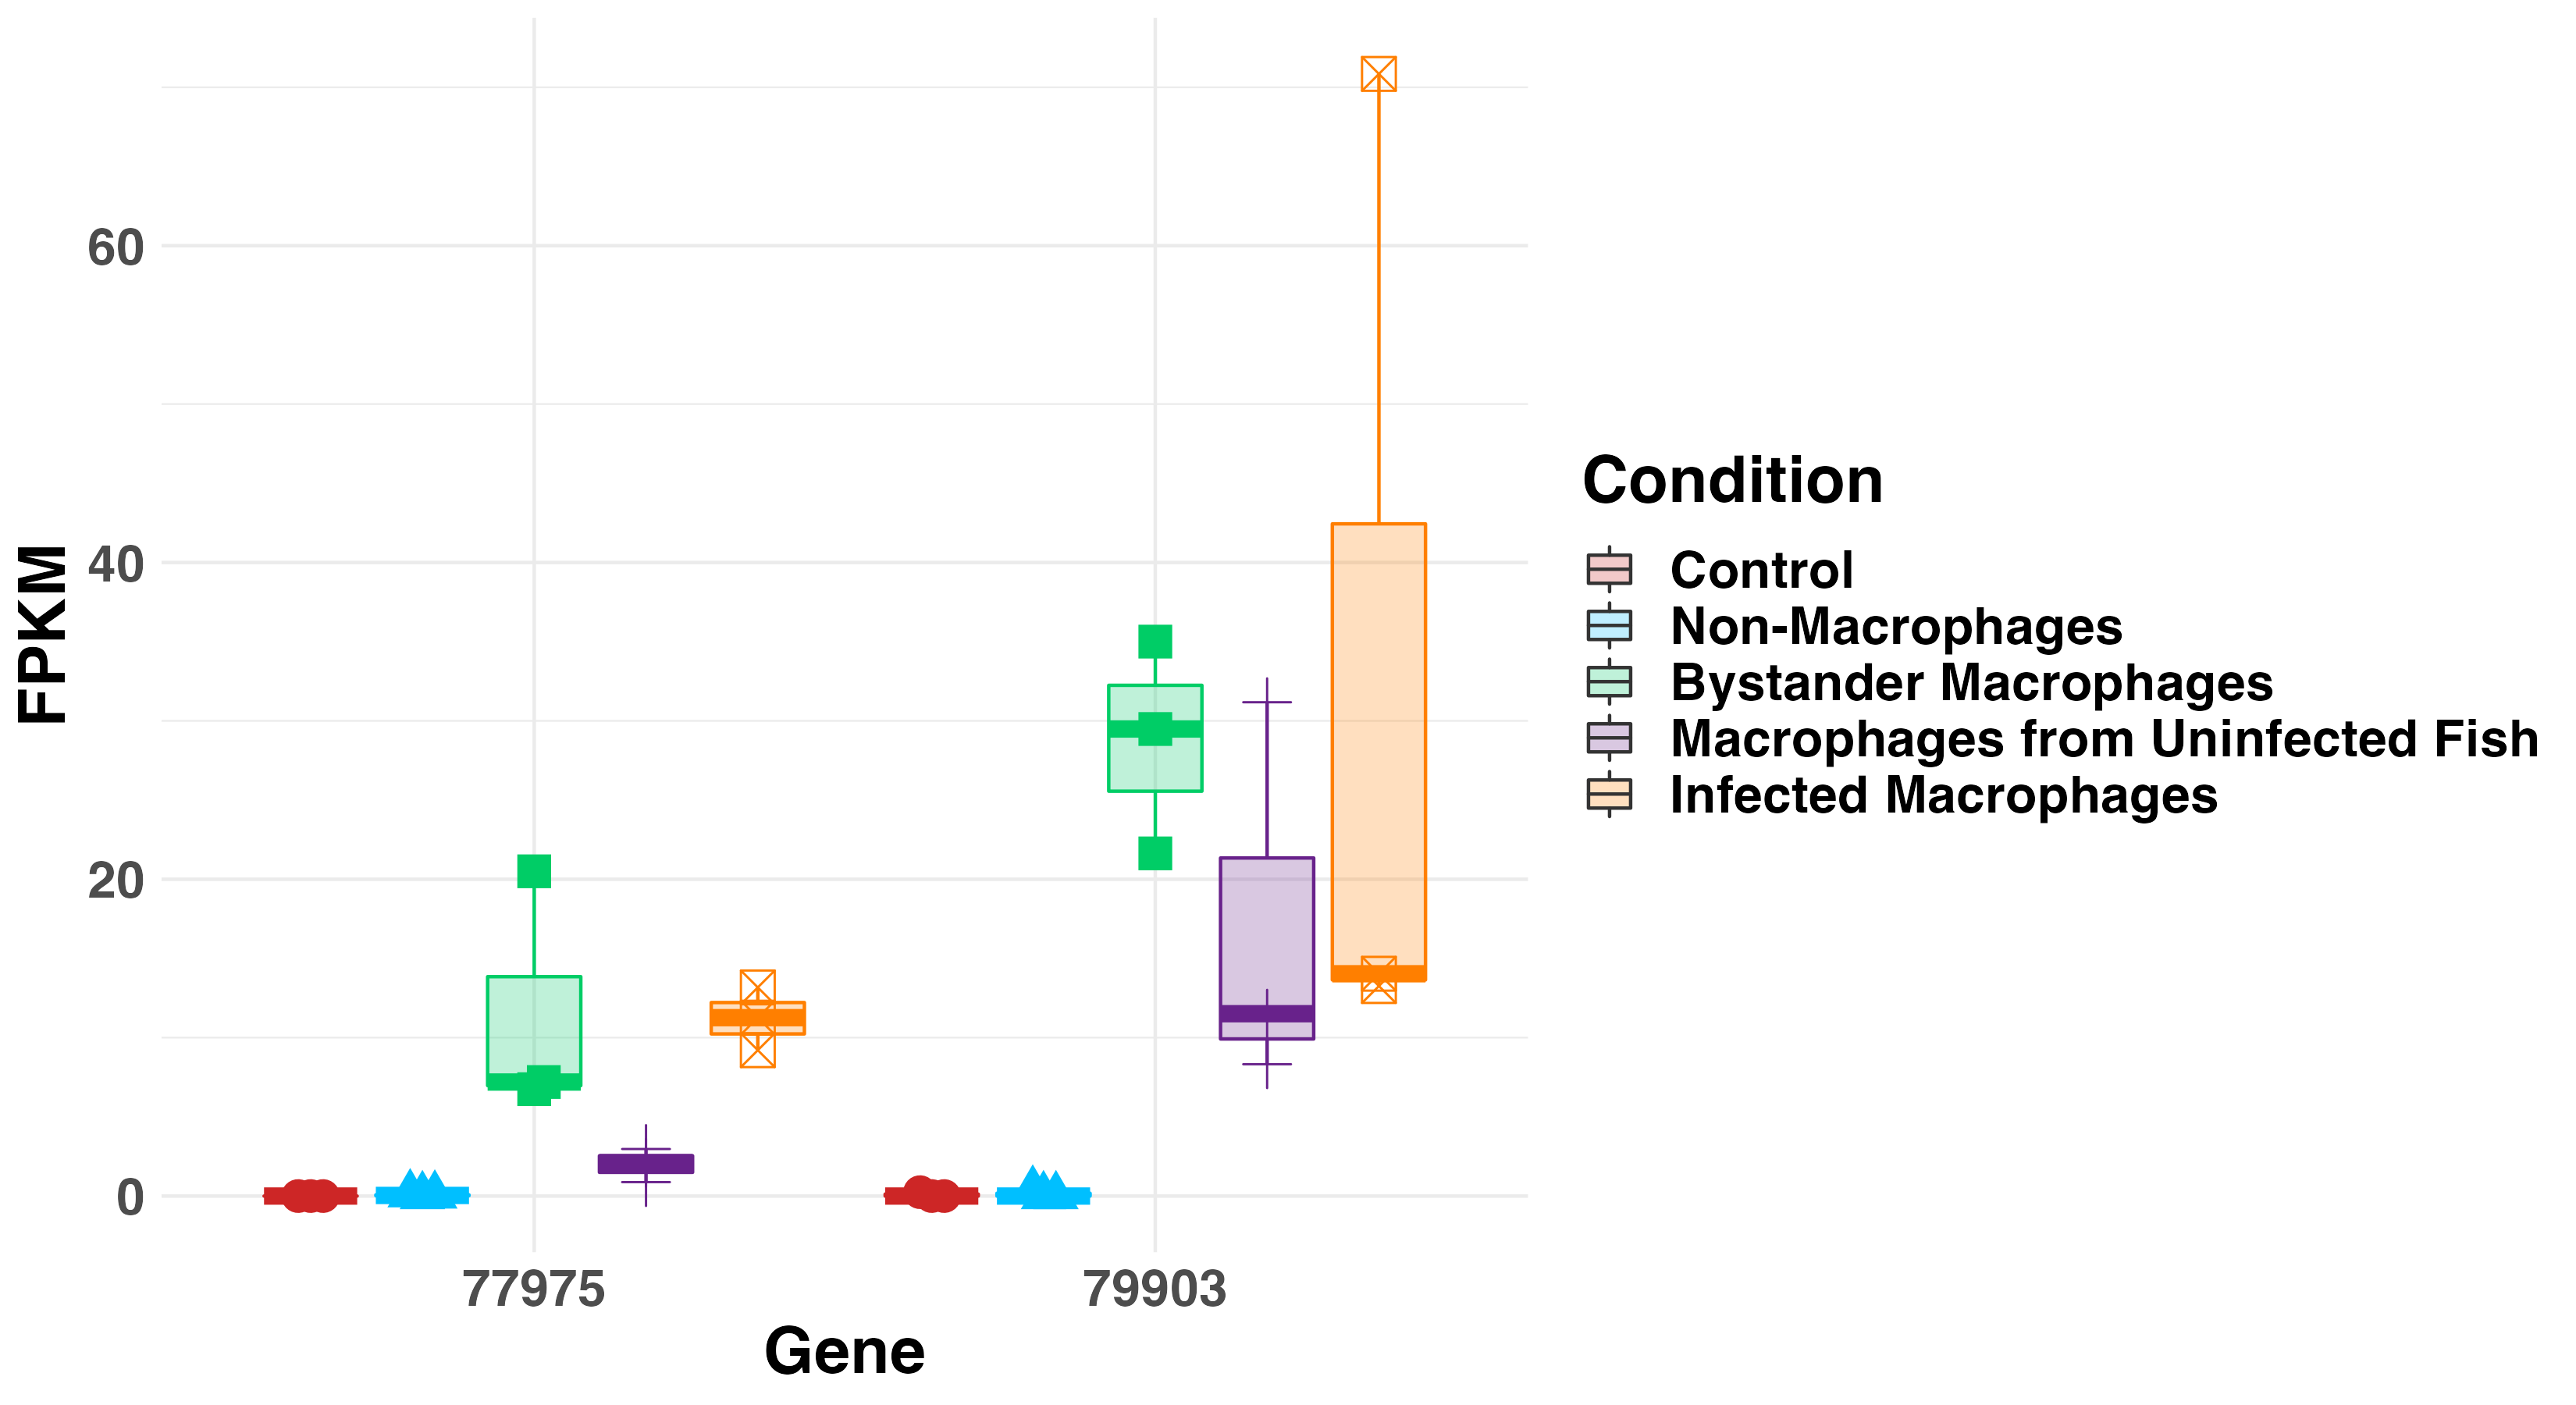
\includegraphics[width=\textwidth]{images/mincle_expression.png}
\caption{Comparison of the expression profiles of two of the putative MINCLE homologs, ENSDARG00000077975 and ENSDARG00000079903 based on existing RNA\hyp{}seq datasets in the Tobin lab. Both of these genes are generally restricted to macrophages and are induced by the presence of mycobacterial infection, an effect exceptionally notable for 77975. This provides some evidence that these genes are regulated by mycobacterial infection and may be playing some role in this context.}
% Provide a label so we can cross\hyp{}reference it from the tex
\label{figure:mincles}
\end{figure}

In the zebrafish itself, I would actually propose to take a few steps backward and return to a mosaic\hyp{}based screening approach. While the long\hyp{}term goal should be to generate a full locus\hyp{}spanning deletion of 77975 and 79903, it may be worthwhile to use the zebrafish as a screening platform to determine the potential contributions of these two genes separately and together in the angiogenesis phenotype and CRISPR/Cas9 ribonucleoprotein injections allow for such rapid screening and planning for whether it makes sense to invest the time and energy in generating a full deletion mutant. Given the unlikelihood of being able to ever generate a crossover event to combine the two existing mutations, some alternative approach is clearly going to be required and this seems like a suitable place to start in pursuit of the zebrafish TDM receptor(s). These two genes make for especially compelling candidates as they are macrophage\hyp{}specific and are induced by infection, even in bystander macrophages (\autoref{figure:mincles}). 

\begin{singlespace}
\begin{center}
\begin{table}
\caption{Putative zebrafish MINCLE homologs with key details about their native structure and mutants that have been generated thus far.}
\label{zfmincs} \tabularnewline
\vspace{0.5cm}
\begin{tabular}{|l|l|l|l|l|l|}
\hline
\thead{Gene ID} & \thead{56379} & \thead{79903} & \thead{77975} \tabularnewline
\hline
Length & 263 & 263 & 170 \tabularnewline
\hline
CRD & kEPNn & gEPNn & gEPNn \tabularnewline
\hline
Identity & 41\% & 42\% & 42\% \tabularnewline
\hline
Similarity & 50.7\% & 53.3\% & 60.3\% \tabularnewline
\hline
Mutation & ::13 & ::13 & $\upDelta$8 \tabularnewline
\hline
Site (a.a.) & 43 & 207 & 108 \tabularnewline
\hline
RMSD & 1.34 & 1.17 & 0.87 \tabularnewline
\hline
TM\hyp{}score & 0.86 & 0.85 & 0.86 \tabularnewline
\hline
Reference Coverage & 95\% & 91\% & 92\% \tabularnewline
\hline
Target Coverage & 91\% & 96\% & 100\% \tabularnewline
\hline
\end{tabular}
\end{table}
\end{center}
\end{singlespace}

Additionally, it may be of some use to study the specific human MINCLE\hyp{}mycobacteria interactions in the context of a whole immune system. Thus, going forward, it would be logical for future researchers to develop transgenic zebrafish that express human versions of MINCLE and MCL in macrophages and, perhaps, neutrophils, to assess the contributions of the human protein to conserved responses. This may also help to clarify some of the conflicting data in the literature around the role of MINCLE by using an overexpression model to capture the effect of excess MINCLE signaling. In the long term, gene replacement of the native MINCLE\hyp{}like homolog with the human MINCLE would allow for a more authentically humanized model of macrophage biology within the zebrafish. Use of this as a complementation strategy if we can identify the zebrafish MINCLE would also serve as a more comprehensive humanized model to study the MINCLE\hyp{}specific contributions to angiogenesis and bacterial control.

\begin{figure}
\centering
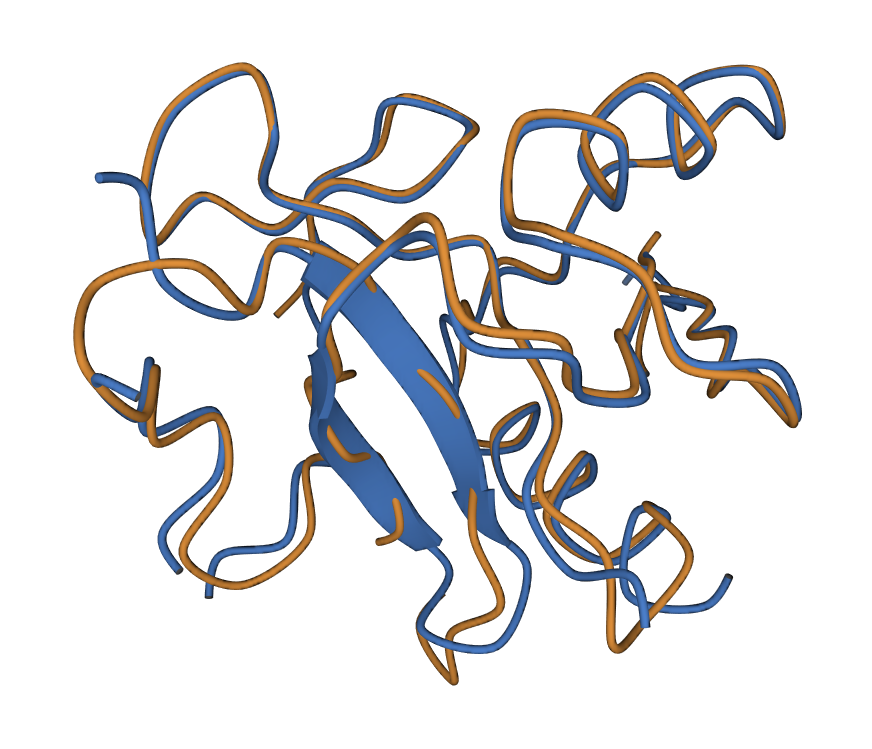
\includegraphics[width=\textwidth]{images/56379_align.png}
\caption{Pairwise structural alignment of the carbohydrate recognition domains of the human MINCLE and zebrafish 56379 showing strong structural overlap indicative of a common structure in excess of the amino acid level similarity.}
% Provide a label so we can cross\hyp{}reference it from the tex
\label{figure:56379}
\end{figure}

\begin{figure}
\centering
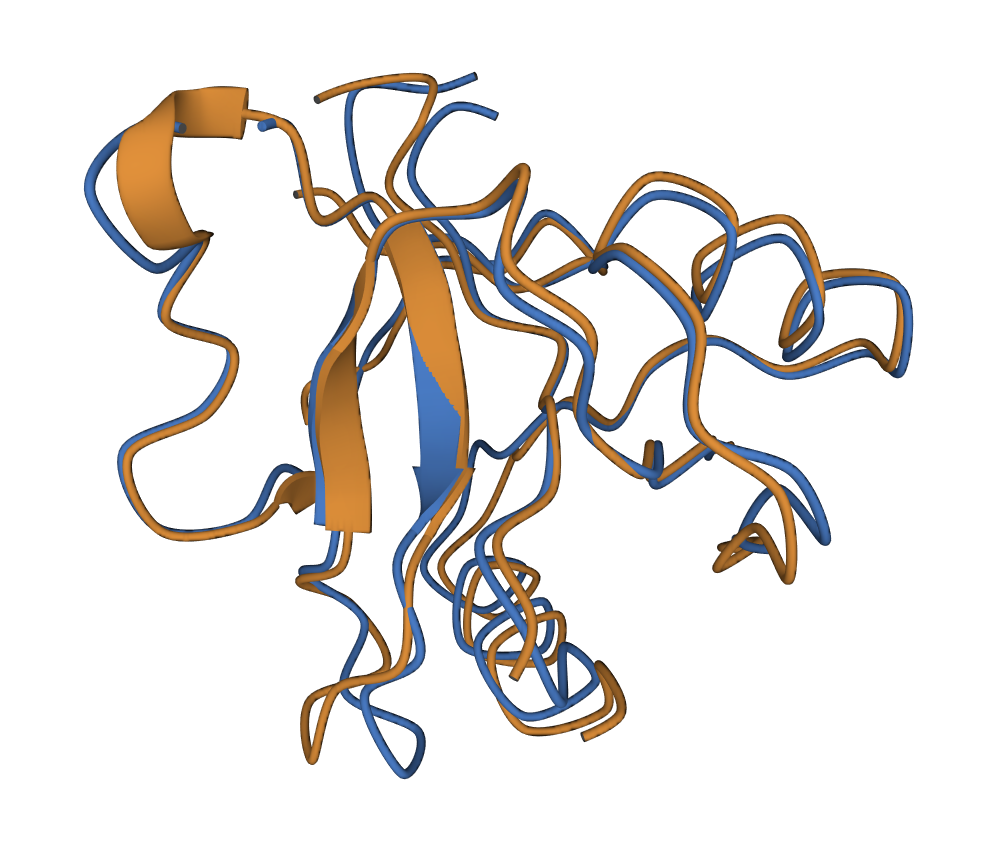
\includegraphics[width=\textwidth]{images/79903_align.png}
\caption{Pairwise structural alignment of the carbohydrate recognition domains of the human MINCLE and zebrafish 79903 showing strong structural overlap indicative of a common structure in excess of the amino acid level similarity.}
% Provide a label so we can cross\hyp{}reference it from the tex
\label{figure:79903}
\end{figure}

\begin{figure}
\centering
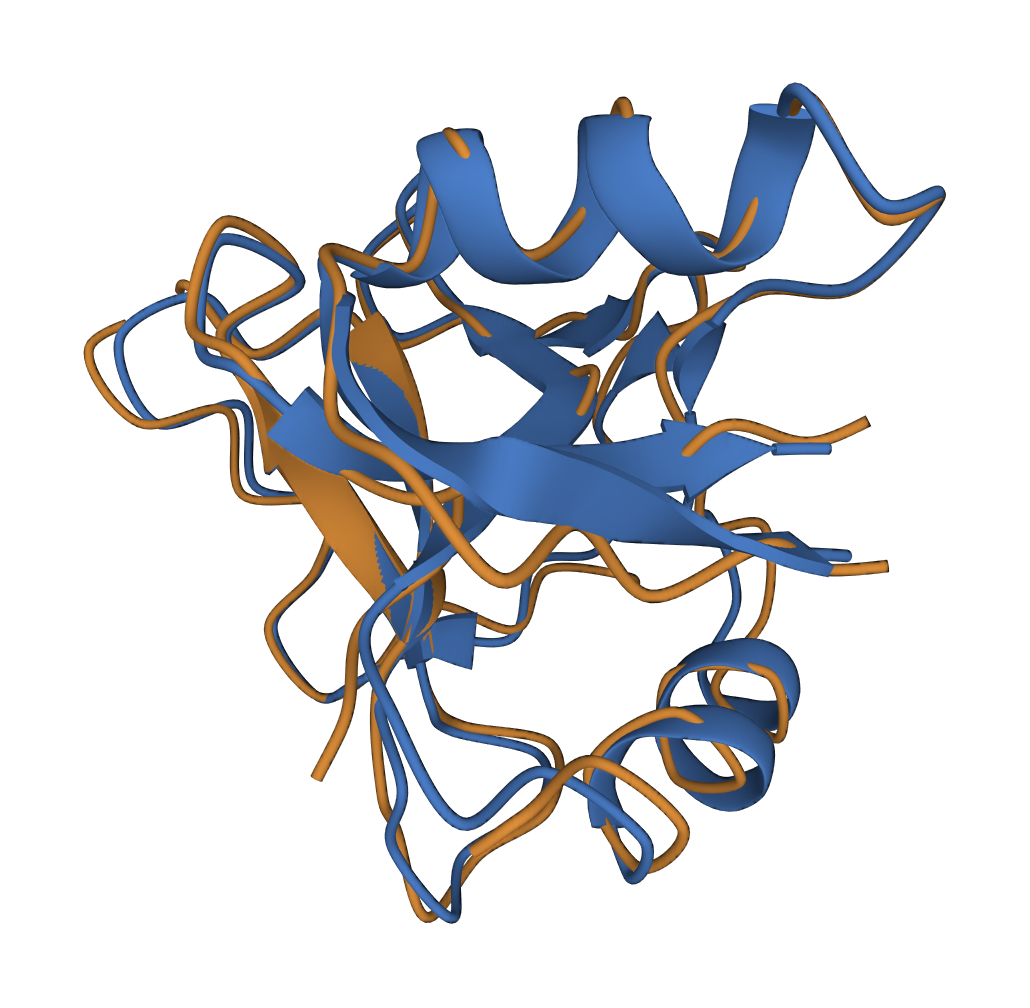
\includegraphics[width=\textwidth]{images/77975_align.png}
\caption{Pairwise structural alignment of the carbohydrate recognition domains of the human MINCLE and zebrafish 77975 showing strong structural overlap indicative of a common structure in excess of the amino acid level similarity.}
% Provide a label so we can cross\hyp{}reference it from the tex
\label{figure:77975}
\end{figure}

While these proteins were originally chosen based on the criteria listed in \autoref{minctab}, the emergence of AlphaFold has allowed for highly accurate structure prediction for any sequence of amino acids, which has allowed for subsequent structural comparisons between these genes and the human MINCLE extracellular domain that indicates a strong similarity between them based on TM\hyp{}score and overall structural alignment (\autoref{zfmincs}) \citep{Jumper2021}. I have conduced these pairwise alignments for each of the three genes of interest and this analysis indicates very high degrees of structural similarity among them, suggesting that they are strong candidates to bind similar ligands (\autoref{figure:56379}, \autoref{figure:79903}, \autoref{figure:77975}). However, this is disadvantaged by the fact that many carbohydrate recognition domains from diverse C\hyp{}type lectins share major structural features, so these data must be taken into consideration with the primary sequence information to draw any meaningful conclusions (\autoref{zfmincs}). Nevertheless, the access to structural information is immensely useful in characterizing some of these candidates and may allow for a better understanding of the features required for binding to TDM.

\section{Integration of Hypoxia Signaling}\label{hypoxia}

The literature is replete with descriptions of HIF\hyp{}1$\upalpha$ regulation of VEGFA production and signaling; the logical means by which to alleviate local hypoxia is through the recruitment of vasculature carrying oxygenated blood. This allows angiogenesis to occur when necessary and for the vasculature to remain quiescent under homeostatic conditions, where intravital oxygen concentrations are maintained at a high level. However, in areas of pathogen invasion, tumor growth, or tissue damage, the local oxygen concentration can fall, triggering the activation of the HIF\hyp{}1$\upalpha$ signaling pathway in neighboring cells. HIF\hyp{}1$\upalpha$ is an oxygen\hyp{}sensing protein that is expressed and rapidly degraded under normoxic conditions but stabilized under hypoxia. Under standard oxygen concentrations, two classes of regulatory proteins mediate prolylhydroxylation and proteosomal degradation of HIF\hyp{}1$\upalpha$ in a process dependent on molecular oxygen \citep{Corcoran2016, Hong2004, Masoud2015}.

Alternatively, HIF\hyp{}1$\upalpha$ can be induced through transcriptional alterations in the homeostatic stoichiometry of HIF\hyp{}1$\upalpha$ itself and the two families of regulatory proteins, PHD and FIH. This allows HIF\hyp{}1$\upalpha$ to be induced under normoxic conditions, the presumed whole\hyp{}body state of the zebrafish larva \citep{Ellertsdottir2010}. This normoxic activation has been found to be important for myeloid immune responses, including those downstream of MINCLE activation, and may play an important role especially in the early signaling events of mycobacterial infection \citep{Nishi2008, Schatz2016, Schoenen2014, Thompson2017}. 

In the environment of the granuloma, both the host and pathogen must adapt to reduced oxygen tension \citep{Prosser2017}. Mycobacteria can temporarily revert into a non\hyp{}replicating state known as persistence, but this is not a viable strategy for long\hyp{}term evolutionary success \citep{Ehrt2018, Stewart2003, Manabe2000, Pandey2008, zuBentrup2001}. However, during persistence, the bacteria are extremely difficult to kill as most antitubercular drugs are only effective on replicating bacteria \citep{Veatch2018}. Even during active growth, the bacteria and associated host cells must alter their metabolism to accommodate for reduced oxygen availability, with important consequences for host immunity \citep{Harper2012, Tsai2006, Prosser2017, Rustad2009, Galagan2013}. Despite our superficial knowledge about the importance and contributions of hypoxia in the lifestyle of \textit{M. tuberculosis}, we do not have a clear means to genetically manipulate these responses or to differentiate the roles of hypoxia \textit{per se} from the activity of HIF\hyp{}1$\upalpha$ signaling. Thus, going forward, new tools are going to be required to study not only the contributions of HIF\hyp{}1$\upalpha$ in mycobacterial infections, but also the broader consequences of this pathway in macrophage physiology and how those contributions might intersect with the role of NFAT in inducing VEGFA production and angiogenesis in this environment.

\subsection{HIF for HIF's Sake}\label{hif4hif}

\citep{, , , , , Woods2022}

HIF\hyp{}1$\upalpha$ has only recently been intensively studied in the context of tuberculosis, with many of the foundational studies coming from Philip Elks's lab in the zebrafish\footnote{There are also described roles for HIF\hyp{}2$\upalpha$ in regulating certain aspects of neutrophil biology during mycobacterial infection, but this is beyond the scope of the presently proposed work \citep{Thompson2014, Elks2015}.}. These early studies utilized both dominant\hyp{}negative and dominant\hyp{}active versions of the zebrafish \textit{hif1ab}\footnote{As is all too common, but rarely quite so penetrant, zebrafish have two copies of all of the HIF\hyp{}$\upalpha$ subunits, making for an expansive coding space for these genes in the zebrafish genome and each copy appears to have some distinct effects, making for both opportunity and frustration \citep{Elks2015}.} to modulate the activity of this pathway, particularly in neutrophils, and have found that activation of HIF\hyp{}1$\upalpha$ prolongs inflammation and improves mycobacterial clearance, suggesting that at early time points, HIF\hyp{}$\upalpha$ plays a protective role in infection \citep{Elks2011, Elks2013, Hammond2020}. These protective effects also extend to macrophages, where HIF\hyp{}1$\upalpha$ stabilization enhances bacterial killing, presumably related to alterations in metabolism \citep{Knight2018, Zenk2021}. However, it has also been shown that HIF\hyp{}1$\upalpha$ prolongs alveolar macrophage survival after injury, an effect that, if present during tuberculosis, may actually exacerbate disease due to the maladaptive nature of alveolar macrophage responses; prompt necrosis of these cells would likely be more beneficial than their continued survival as a protective niche for the bacteria \citep{Woods2022, Leemans2001}. Other studies have also identified an essential role for HIF\hyp{}1$\upalpha$ in both IFN\hyp{}$\upgamma$ responses and TNF\hyp{}$\upalpha$ expression, both of which are essential for bacterial control \citep{Braverman2016, Lewis2019, Flynn1993, Flynn1995}. However, unlike the responses in macrophages, HIF\hyp{}1$\upalpha$ stabilization in T cells inhibits effective cytotoxic responses, impairs host immunity, and induces disease tolerance, so it is clear that the balance of effects is critical to the determination of the overall role of HIF\hyp{}1$\upalpha$ during infection \citep{Liu2022b, Tzelepis2018}.

\begin{figure}
\centering
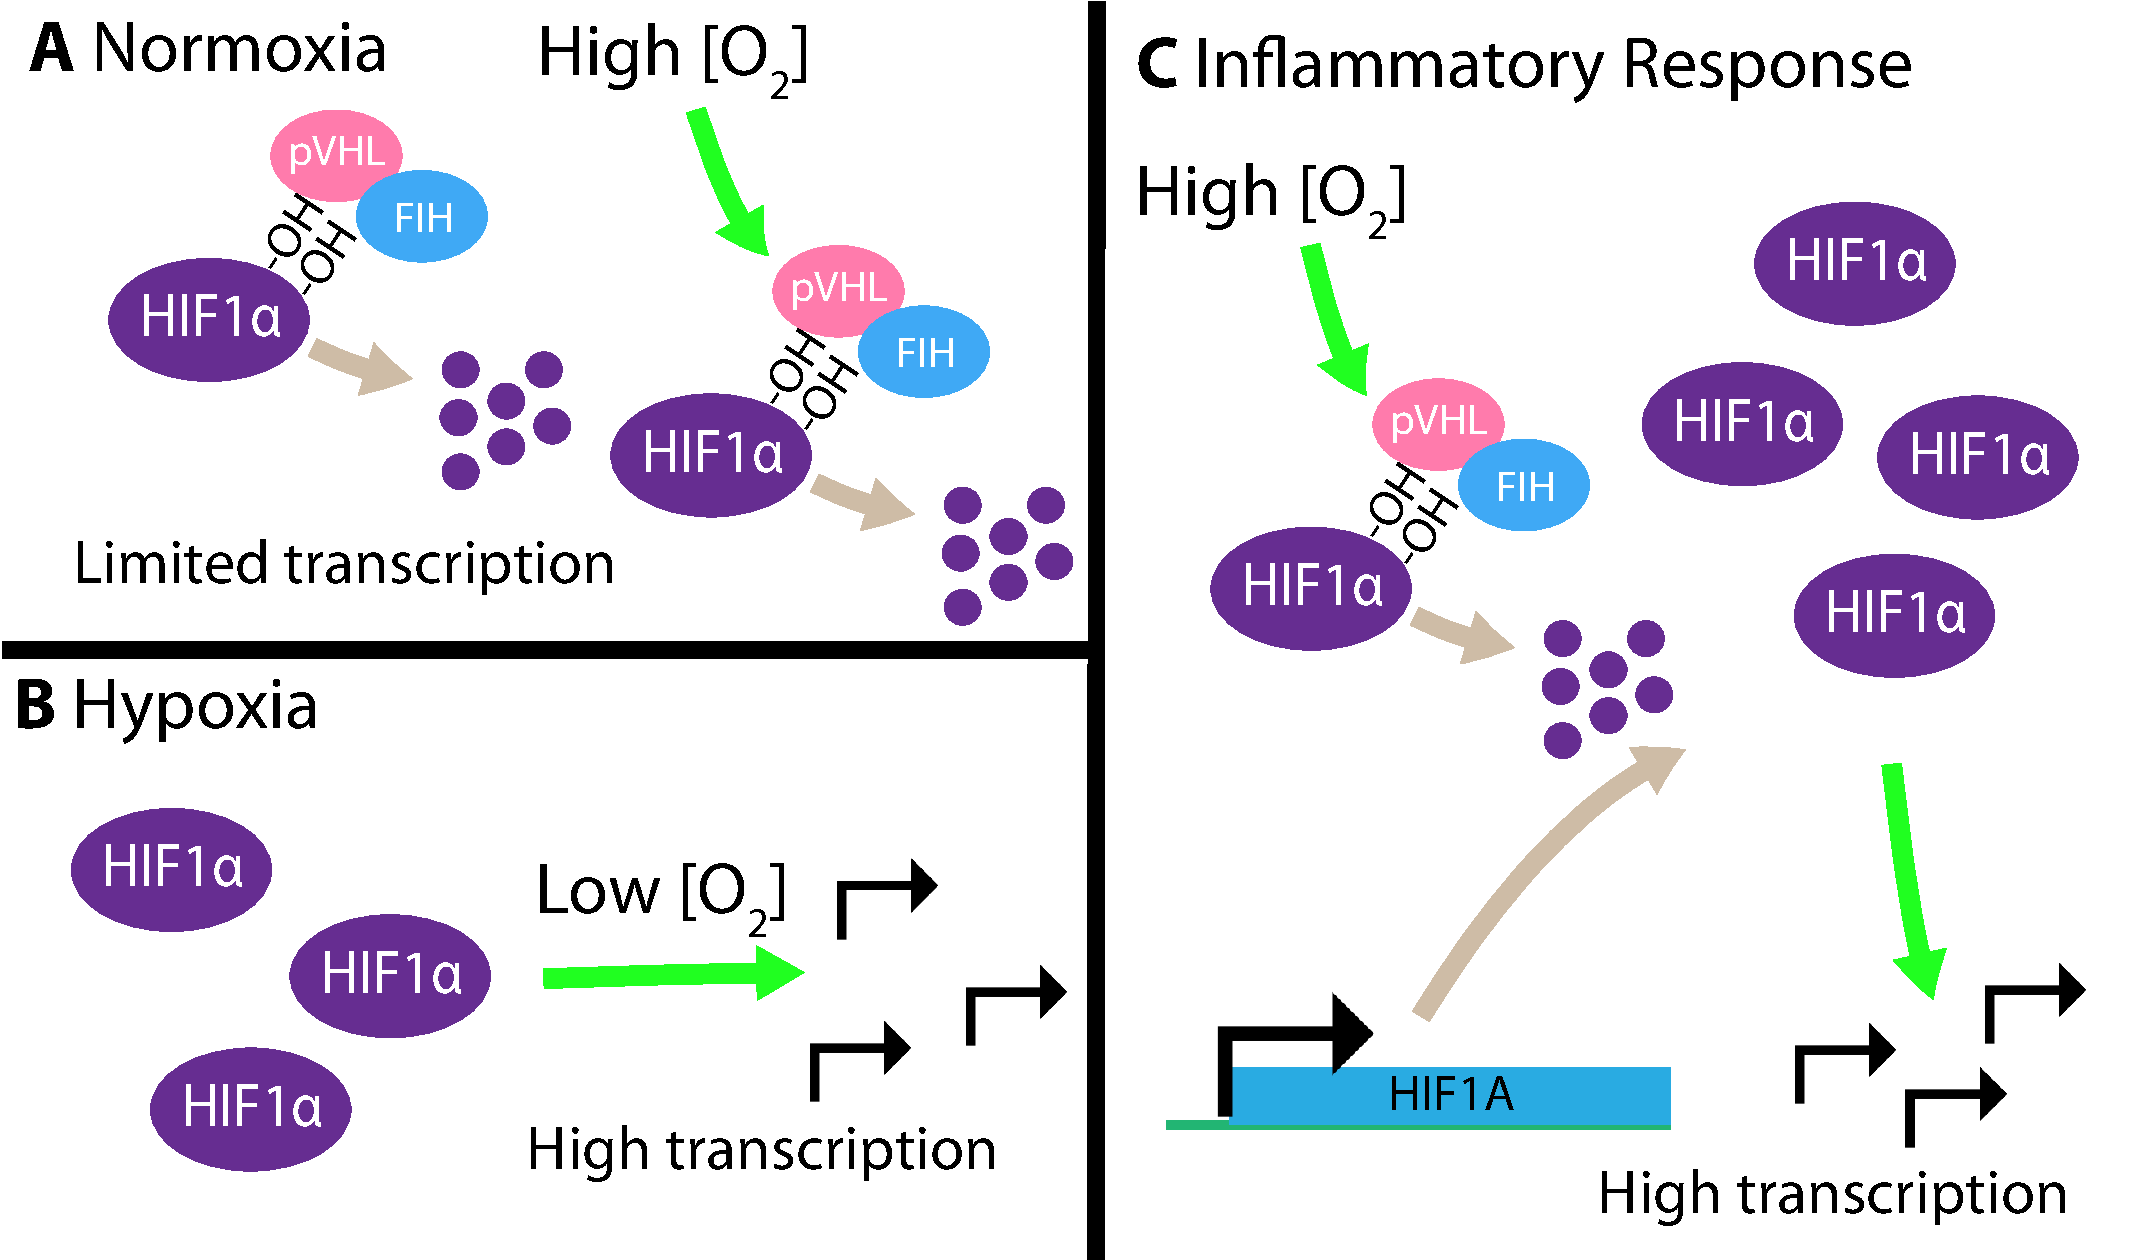
\includegraphics[width=\textwidth]{images/hifreg.pdf}
\caption{Schematic demonstrating the different states of HIF\hyp{}1$\upalpha$. (A) shows the standard normoxic state of HIF\hyp{}1$\upalpha$, where it is rapidly degraded by oxygen\hyp{}dependent enzymes; (B) these enzymes are inhibited in hypoxia, leading to HIF\hyp{}1$\upalpha$\hyp{}dependent transcription. (C) Immunological stimuli can result in HIF\hyp{}1$\upalpha$ transcription, leading to functional activation even in the absence of overt hypoxia.}
% Provide a label so we can cross\hyp{}reference it from the tex
\label{figure:hif}
\end{figure}

More generally, HIF\hyp{}1$\upalpha$ mediates both priming and responding to diverse insults. Hypoxia is able to induce the expression of \textit{TLR2} and \textit{TLR6}, which are important for broad responses to various infections, including \textit{M. tuberculosis} \citep{Kuhlicke2007}. However, once induced by the pathogen itself, HIF\hyp{}1$\upalpha$ is a critical inducer of \textit{IL1B} and IL\hyp{}1$\upbeta$ which, as we have seen is an important dimension of the host defense against mycobacterial infections \citep{Ogryzko2019}. Indeed, HIF\hyp{}1$\upalpha$ is able to be activated indirectly by C\hyp{}type lectin signaling, suggesting it may play a role in major antifungal and mycobacterial responses although the precise consequences of this mechanism of activation are still being worked out \citep{Elder2019, Friedrich2017}. As might be expected, genetic stabilization of HIF fosters more robust protective responses against multiple pathogens, paralleling findings from mycobacteria and making this a potential target for agonism as a means of fostering broad immune defense as well as trained immunity \citep{Schild2020}. This extends to macrophages specifically, which can exert improved killing of \textit{M. tuberculosis} after HIF\hyp{}1$\upalpha$ activation \citep{Li2021}. Different physiological conditions within the host can impair HIF activation and HIF\hyp{}dependent responses, including high blood glucose, adding a potential dimension to the immunosuppression experienced by many diabetics \citep{Teran2022}. On the other hand, glucose influx is important for initial glycolysis initiation, so there is likely to be some degree of Goldilocks effect where the right amount of glucose can facilitate glycolytic metabolism but too much overwhelms the system and too little starves the cells \citep{Stunault2018}. Other studies have implicated HIF\hyp{}1$\upalpha$ signaling in inhibiting macrophage necrosis in mycobacterial granulomas, indicating that this signaling pathway may exert some protective effects in particular contexts, although this study focused on \textit{M. avium} granulomas, which differ in some respects from \textit{M. tuberculosis} granulomas \citep{Cardoso2015}.

Alterations in metabolism through HIF\hyp{}1$\upalpha$ also underly so\hyp{}called ``trained immunity\footnote{Trained immunity is a process in which the innate immune system is primed to respond to future insults more effectively. This akin to the way that vaccinations prime the adaptive immune system, but through a completely different set of mechanisms and is non\hyp{}specific, allowing for broad protection against diverse insults.},''. The induction of aerobic glycolysis within macrophages primes them to respond more vigorously to future insults, an effect that appears to be able to last weeks or months \citep{Cheng2014}. As HIF\hyp{}1$\upalpha$ is a known mediator of IL\hyp{}1$\upbeta$ induction, it appears that increased transcription in the absence of post\hyp{}translational processing to increase the pool of latent pro\hyp{}IL\hyp{}1$\upbeta$ is one of the mechanisms by which this process is able to work \citep{Arts2018}. Trained immunity may even serve as a transgenerational mechanism of protection against insults \citep{Katzmarski2021}, although this is controversial \citep{Kaufmann2022, Katzmarski2022}. The synthesis of the effects on metabolism with effects on macrophage biology and interactions with the surrounding stroma in mediating some of the effects of trained immunity still require a great deal of investigation, although this is certainly yet another realm where major families of immunologically relevant transcription factors surely play some role. It is known that the BCG vaccine is able to induce broad trained immunity, which is a potential mechanism by which BCG is thought to be able to protect against both bladder cancer, and, perhaps, COVID\hyp{}19 and other respiratory viruses \citep{Arts2016, Arts2018, Covian2019, vanPuffelen2020, ONeill2020}.

This work nicely complements work from Didier Stainier's lab, which used a combination of \textit{hif1aa} and \textit{hif1ab} mutant zebrafish and new macrophage\hyp{}specific transgenic tools to manipulate the HIF\hyp{}1$\upalpha$ signaling pathway and found that this pathway, specifically in macrophages, was critical for mediating developmental angiogenesis. Unlike the behaviors seen in neutrophils, specific expression of even a wild\hyp{}type \textit{hif1ab} in macrophages was toxic to the cells and rendered them impotent\footnote{It is difficult to contextualize all of these results; mRNA injection of \textit{hif1ab} results in a discrete set of less\hyp{}severe phenotypes than transgenic expression of this cDNA strictly within macrophages? Additionally, this expression is clearly an impediment to immune responses but the Elks lab has repeatedly seen protection from whole\hyp{}organism HIF\hyp{}1$\upalpha$ stabilization and overexpression in neutrophils, arguing that there are confusing layers of additional regulation or compensation that we do not presently understand that stand in the way of effective transgenic control of this pathway.} \citep{Gerri2017}. This toxicity is likely due to sequestering of important binding partners, but may be due to metabolic changes that leave the cells unable to produce sufficient ATP, albeit by two divergent mechanisms -- wild\hyp{}type \textit{hif1ab} may produce a strict reliance on glycolysis while dominant\hyp{}negative \textit{hif1ab} may force oxidative phosphorylation at rates exceeding the ability to produce pyruvate. A clearer understanding of the precise mechanism of this transgene\hyp{}specific macrophage toxicity would likely reveal interesting new dimensions to the HIF\hyp{}1$\upalpha$ pathway in macrophages\footnote{Other hypotheses include the overexpressed HIF\hyp{}1$\upalpha$ sequestering essential cofactors from other proteins, breaking the stoichiometry of essential protein:protein interactions, or some other mechanism. That does not explain why mRNA overexpression and genetic knockout are both better tolerated, however.}. This evokes an important function of this pathway in these cells that current tools remain unable to address. 

HIF\hyp{}1$\upalpha$ signaling is also implicated in various aspects of tumor biology and, as mentioned in \autoref{cancerang}, is important in mediating the angiogenic response in cancer. It also plays important functions in other aspects of cancer biology, including modulating tumor pH and the extracellular matrix \citep{Dayan2008}. These studies within tumors have also revealed interesting layers of transcriptional regulation within the HIF\hyp{}1$\upalpha$ regulon and the functional differences between FIH and PHD, where PHD proteins are very strictly dependent on environmental oxygen while FIH has a much higher affinity for oxygen and can operate even at relative hypoxia. Given the different domains targeted by these proteins, HIF\hyp{}1$\upalpha$ can exert biphasic effects at varying oxygen tension, with certain genes upregulated at modest hypoxia and additional genes induced under severe hypoxia \citep{Dayan2008}. Such gradients of response may be critical to understanding this pathway during mycobacterial infection, where the timing of these changes in relative oxygen concentration may reflect distinct stages of disease.

To further the study of the HIF pathway in the context of mycobacterial infection in the zebrafish, a set of new tools should be made: one is a set of reporter constructs to better identify both hypoxic and transcriptional induction of \textit{hif1ab} in macrophages and the other is a conditional approach to the expression of dominant negative and dominant active versions of HIF\hyp{}1$\upalpha$ in macrophages, potentially enabling new cell\hyp{}autonomous understanding of the role of this pathway in mycobacterial pathogenesis and angiogenesis.

Previous work in our lab using \textit{in situ} hybridization for \textit{phd3} mRNA revealed the upregulation of this gene surrounding the mycobacteria, indicating hypoxia \citep{Oehlers2015}. The Elks lab generated a transgenic line using a bacterial artificial chromosome containing the promoter for \textit{phd3} that expresses GFP \citep{Santhakumar2012}, which serves as a useful spatial and temporal readout for HIF\hyp{}1$\upalpha$ transcription factor activity across different tissues. However, this tool is unable to distinguish between normoxic and hypoxic activation or different cell types, so new tools are required to better address these questions.

During conditions of hypoxia, HIFs are degraded through hydroxylation in the oxygen dependent degradation domain (ODD) that contains two proline residues that are hydroxylated by PHD proteins, leading to proteasomal degradation. This ODD has been shown to be both necessary and sufficient to direct oxygen\hyp{}dependent degradation, so it seems reasonable to use a macrophage\hyp{}specific promoter to drive expression of ODD linked to a fluorescent protein as a reporter for granuloma hypoxia. This would be stabilized at low oxygen concentration while being constitutively degraded under normoxia. This would allow for a clearer report of the degree of present hypoxia and complement existing tools, including hypoxyprobe \citep{Cousins2016, Huang1998}. If this tool alone were to be sufficient to induce macrophage toxicity, then an alternative approach could be taken to induce this transgene only when needed using degradation domains or inducible promoters, such as the \textit{hsp70l} heat shock\hyp{}inducible promoter. Further discussion on degradation domain regulation will be provided shortly.

In parallel, a reporter is needed to provide a readout of normoxic activation of HIF\hyp{}1$\upalpha$, which is predominantly thought to be regulated at the transcriptional level and through accumulation of the citric acid cycle intermediates $\upalpha$\hyp{}ketoglutarate and succinate \citep{Meng2018, Palazon2014, Tannahill2013, Williams2018}. Therefore, either ectopic expression or direct protein fusion strategies would be appropriate to the study of this pathway. If some promoter could be identified that responded comparably to the native \textit{hif1ab} promoter or a CRISPR\hyp{}mediated knockin could be generated, this would be a useful reporter of transcription\hyp{}level induction of HIF\hyp{}1$\upalpha$, a process likely relevant to inflammatory responses during infection. Alternatively, a bacterial artificial chromosome\hyp{}based transgenic could be constructed, which might be easier than screening for a knockin while more faithfully recapitulating the expression pattern than a promoter\hyp{}based transgenic. This, in tandem with the previously mentioned ODD transgenes would allow for a more thorough dissection of the relative contributions of hypoxia \textit{per se} and the activity of HIF\hyp{}1$\upalpha$. An additional approach would be to develop biosensors that can detect either succinate or $\upalpha$\hyp{}ketoglutarate, examples of which already exist in the literature \citep{Liu2017b, Suzuki2021, Luddecke2017}. Developing macrophage\hyp{}specific sensors to detect these HIF\hyp{}1$\upalpha$\hyp{}inducing metabolites would offer another means to assess these effects while also offering a secondary approach to understand the mechanisms of HIF\hyp{}1$\upalpha$ induction during immune responses to mycobacterial infection. 

As previous transgenic attempts have failed, the expression of dominant negative\hyp{}\textit{hif1ab} and dominant active\hyp{}\textit{hif1ab} in macrophages will require new approaches. It seems that misregulation of HIF\hyp{}1$\upalpha$ signaling results in some sort of developmental toxicity in the macrophage, so it is critical that HIF is only modulated in the time and place where it is most relevant. Thus, using established estradiol\hyp{}responsive constructs, a set of fish should be made expressing dominant negative\hyp{}\textit{hif1ab} and dominant active\hyp{}\textit{hif1ab} covalently linked to ER50 degradation domains, which sequester proteins in the cytosol and target them for degradation except when in the presence of tamoxifen \citep{Miyazaki2012}. This would allow for the creation of HIF\hyp{}modulating transgenes within macrophages that would be expected to have reduced toxicity and allow for time\hyp{}targeted modulation of this pathway. Like the previous tools, this seems especially relevant in the context of mycobacterial granulomas from adult zebrafish, which are known to be hypoxic and more closely resemble human granulomas \citep{Harper2012, Oehlers2015, Rustad2009}. Alternatively, and perhaps even more elegantly, dominantnegative\hyp{}\textit{hif1ab} could be created endogenously, through knock\hyp{}in of a Cre\hyp{}flippable trap cassette into intron 7 or 8; if placed in the ``off" orientation, this would allow for normal HIF\hyp{}1$\upalpha$ activity while induction of macrophage\hyp{}specific Cre\textsuperscript{ERT2} would then allow for macrophage\hyp{}specific activation of a dominant\hyp{}negative version of the protein through introduction of a splice acceptor\hyp{}stop codon\hyp{}polyadenylation sequence. Even further creative approaches could enable tissue\hyp{}specific induction of dominant active HIF\hyp{}1$\upalpha$ through a similar approach by knocking in the remaining cDNA with the hydroxylated proline residues mutated and placing this, too, under control of an invertible \textit{loxP} pair. Such an endogenous approach would also allow flexible pairing with other Cre drivers and simultaneous fluorescent tagging of cells in which the recombination has occurred, allowing these cells to be traced through the course of infection. These are likely to reveal not only new aspects of HIF modulation of angiogenesis, but broader impacts on the overall response to infection, especially given the central role of HIF\hyp{}1$\upalpha$ in altering macrophage metabolism.

\subsection{Macrophage Metabolism in Immunity}\label{metabolism}

Upon activation, macrophages undergo a HIF\hyp{}1$\upalpha$ dependent metabolic switch that corresponds, in part to their longevity and function \citep{Kolliniati2022}. While immediate/early\hyp{}responding macrophages\footnote{In the literature, these are so\hyp{}called ``M1'' macrophages and while useful to acknowledge the inflammatory and activated state of these cells, it is not clear to me nor does it seem likely that macrophages strictly use only one metabolic modus at a time, although many of them are relatively depleted of mitochondria \citep{Biswas2012}.} undergo an inflammatory metabolic switch and begin to utilize aerobic glycolysis for metabolism as a means of rapidly (albeit inefficiently) generating energy, later arrivals and macrophages that survive over longer periods must utilize oxidative phosphorylation to optimize energy consumption over a longer course of immunological response \citep{Shi2019, Kiran2016, Viola2019, Langston2017, Taylor2022}. Thus, while macrophages may initially utilize  bursts of glycolysis for fuel rapid, oxidizing responses, this is an unsustainable mode of metabolism over the long term and these macrophages must either transition to the use of oxidative phosphorylation, disperse, or perish \citep{Odegaard2011, Howard2020}. These metabolic switches are thought to be predominantly regulated by a combination of HIF\hyp{}1$\upalpha$, AKT, and mTOR, although this does not exclude the possibility of other factors influencing these changes, including, perhaps, the NFAT signaling pathway\footnote{Perhaps more likely is that the metabolic state of the cell influences the ability of NFAT to respond -- this will require a long time to fully dissect, appreciate, and synthesize in order to develop the relationships that might exist between the world of possible macrophage responses in the context of their temporal metabolic state.} \citep{Covarrubias2015, Karar2011}. The reason for the present interest in macrophage metabolism is many fold: there is comparatively little known about the immunometabolism of the granuloma itself (at least compared to that of macrophages \textit{sensu stricto}, this process intimately involves HIF\hyp{}1$\upalpha$ signaling (a classical mediator of angiogenesis), and is clearly an important dimension of a variety of protective immune responses and we currently lack a model that integrates what is most likely the most important second messenger of eukaryotes (divalent calcium) with macrophage metabolism, which may allow for a more comprehensive integration of NFAT signaling with these broader changes in macrophage biology. 

The immediate burst of glycolysis additionally generates important metabolic byproducts that can be repurposed for other cellular processes and which might have otherwise been consumed by the citric acid cycle \citep{Viola2019, Kelly2015}. One of the earliest observations on this point evaluated the consequences of loss of function of HIF\hyp{}1$\upalpha$ on the ATP concentrations within myeloid cells and found dramatically reduced levels during inflammation \citep{Cramer2003}. Notable among these are succinate and $\upalpha$\hyp{}ketoglutarate, both of which are able to activate HIF\hyp{}1$\upalpha$ and whose production is agonized by increased HIF\hyp{}1$\upalpha$ activation in a feed\hyp{}forward loop. Wound sites and other sites of insult tend to have reduced oxygen tension, which drives the hypoxic activation of HIF\hyp{}1$\upalpha$ as well. Together these inflammatory and chemical processes induce the production of VEGFA (as well as other cytokines and chemokines) to effectively respond to these stimuli. The macrophage\hyp{}specific induction of HIF\hyp{}1$\upalpha$ can act to mediate critical aspects of both endothelial cell biology as well as further macrophage responses in an autocrine and paracrine manner.

The glycolytic switch that occurs in these first responders is dependent upon and triggered by the inducible nitric oxide synthase (iNOS), which is induced by HIF\hyp{}1$\upalpha$ and generates nitric oxide (NO). Nitric oxide is able to inhibit mitochondrial respiration, reducing the oxidative phosphorylation capacity of the cell and driving it toward alternative means of ATP production, the most compelling of which is aerobic glycolysis. The consumption of glucose by glycolysis without the ability to complete the citric acid cycle results in the accumulation of succinate and $\upalpha$\hyp{}ketoglutarate, which further activate HIF\hyp{}1$\upalpha$. This activation of HIF\hyp{}1$\upalpha$ drives the transcription of glucose transporters and lactate dehydrogenases to block mitochondrial utilization of the pyruvate end\hyp{}product \citep{Russell2019a, GalvanPena2014}. This increase in glucose import has been shown to be important in the pathogenesis of leprosy, although specific experiments with other mycobacterial species would be required to validate the assumed generalizability of this process \citep{Medeiros2016, MontoyaRosales2016, Vance2019}. HIF\hyp{}1$\upalpha$, as we have seen, also induces the expression of numerous cytokines and chemokine, making it an integral part of the overall response to the detection of diverse PAMPs, the model of which is LPS (see \autoref{lps}). As a major mediator of inflammatory responses, the HIF\hyp{}1$\upalpha$\hyp{}dependent glycolytic phenotype of macrophages facilitates rapid, energetically expensive responses to these acute threats but is unsustainable over the long term, forcing a net shift back to oxidative phosphorylation due to both cellular turnover and \textit{in situ} metabolic reprogramming.

In order to switch back to oxidative phosphorylation within a single cell, HIF\hyp{}1$\upalpha$ must be degraded and alternative pathways induced. The net balance of inducible nitric oxide synthase\hyp{}dependent production of nitric oxide and citrulline and arginase\hyp{}dependent production of urea and ornithine appears to be critical for this shift \citep{Palmieri2020, Qualls2016}. This places arginine at the center of tuberculosis immunometabolism and its byproducts -- through nitric oxide and itaconate -- determine key aspects of host immunity. Despite the traditional assignment of \textit{NOS2} as an M1 marker and \textit{ARG1} as an M2 marker, it is known that LPS -- the most classical of M1 stimuli -- can paradoxically induce arginase, which would argue that our current knowledge of the factors that contribute of these different states (if they are to be states as such) is lacking\footnote{In the presence of both iNOS and arginine, relative affinity and expression may play as\hyp{}yet unexplored roles in shaping the overall tone of the immune response on the single cell level. The full categorization of this will require further technology development in single cell proteomics that is far more sensitive than current approaches.} \citep{ElKasmi2008}. A further metabolite in this process, itaconate, has a range of important immunomodulatory and directly antimicrobial properties that have only more recently been explored in the context of tuberculosis immunity \citep{Jinich2022, He2021}. As these processes reflect directly on amino acid metabolism, it is logical that other pathways related to amino acids would contribute to immune processes and indeed, the biosynthesis of other amino acids within macrophages appears to be important for granuloma formation, but the precise roles are relatively unclear.

A great deal of work has been done to study discrete genetic mutants in major genes along these pathways, but the interpretation of these data is challenging. One issue is that much has been done \textit{in vitro} under standard LPS/IFN\hyp{}$\upgamma$ or IL\hyp{}4/IL\hyp{}13 polarization schema or in the mouse, where more comprehensive profiling is possible but is hindered by attempts at placing these changes within dogmatic M1\hyp{}M2 binaries; the knockout of \textit{Arg1} or \textit{Nos2} definitionally changes the cell's location within this dichotomy even if it does not fundamentally change the cellular identity of these populations. A more open\hyp{}minded approach to the functional consequences of mutating critical metabolic genes within macrophages is needed to develop a more lucid understanding of the consequences of shifting macrophage metabolism along a fine gradient. All of these shifts are interwoven with HIF\hyp{}1$\upalpha$ and depend on both inflammatory signals as well as the existence of formal hypoxia and the intersection between these signals has, thus far, been difficult to tease apart.

These metabolic changes are an important aspect of the capacity for macrophages to engage with mycobacteria, although these changes are not necessarily for the betterment of the host. Mycobacteria benefit from phagocytosis by macrophages undergoing glycolysis, even though these are traditionally thought to be more bactericidal \citep{Escoll2019, Mehrotra2014, Shi2019}. This is on account of the induction of fatty acid biosynthesis; mycobacteria utilize lipids as a primary carbon source and the production and uptake of additional lipids by the macrophage, including cholesterol, enhances bacterial growth \citep{Gatfield2000, Nazarova2019, Yan2020}. This is evidenced by the ways in which \textit{M. tuberculosis} subverts cellular metabolism through the use of the tuberculosis necrotizing toxin (TNT), which depletes the macrophage of NAD\textsuperscript{+}, which induces metabolic adaptation within the macrophage to compensate this loss of NAD\textsuperscript{+} and transition back to oxidative phosphorylation in those instances where the macrophage does not simply die \citep{Howard2020}. 

The products and intermediates in glycolysis have known antimycobacterial activity, including nitric oxide and prostaglandins, making macrophage metabolism a delicate balance between the bacteria's ability to manipulate the macrophage into a permissive state while minimizing the risks from these potentially antimicrobial responses \citep{OsadaOka2019}. However, these metabolic changes also induce the production of IL\hyp{}1$\upbeta$, which has known protective activity against mycobacteria, suggesting that macrophages are able to utilize strategies to overcome these layers of bacterial subversion \citep{Corcoran2016, Ogryzko2019, Fremond2007, Shi2019}. Another aspect of this is wherein macrophage accumulate lipids for their own utility while barring bacterial access to these resources by the sequestration of them within cytosolic lipid droplets \citep{Laval2021, Knight2018}. The limitation of macrophage access to cholesterol through various means has the potential to induce forms of nutritional immunity against the bacteria and shift macrophages into more bactericidal states \citep{Babunovic2022, Pandey2008, Yang2014c}. A more comprehensive evaluation of the overall metabolic drivers in macrophages during these immune responses is still very much a work in progress with many questions remaining about how mycobacteria are able to alter macrophage metabolic status for their benefit and compensatory mechanisms within the macrophage to overcome such subversion. Many of these processes may be mediated by the induction of PPAR\hyp{}$\upgamma$, which is able to induce the import of cholesterol and other lipids and is known to be induced in granuloma macrophages, offering a complementary metabolic pathway to further define in the context of mycobacterial infection \citep{Chawla2001}.

Under sustained immunological stimulation during hypoxia, such as that found in the tuberculous granuloma, metabolic reprogramming toward oxidative phosphorylation occurs within macrophages that corresponds to downregulation of HIF\hyp{}1$\upalpha$ \citep{Wilson2019, Mehrotra2014}. This raises a potent conflict between the production of VEGFA, the M2\hyp{}like identity of many of the VEGFA\hyp{}expressing granuloma macrophages, and the downregulation of the presumptive master regulator of VEGFA, HIF\hyp{}1$\upalpha$. Some aspects of this conflict between the paradoxical decrease in HIF\hyp{}1$\upalpha$ signaling and the increase in VEGFA production can now be resolved based on the present work, which presents an alternative model of a C\hyp{}type lectin receptor\hyp{}NFAT transduction pathway able to induce the transcription of VEGFA independent of hypoxia\footnote{This is evidenced by the induction of angiogenesis in the larval zebrafish, which is perfused with oxygen, and the induction of VEGFA in THP\hyp{}1 macrophages, which are cultured under 21\% O\textsubscript{2} in air.}. It may be that under this model the metabolic status of the macrophages is ultimately unimportant for VEGFA production or there are additional layers of intersectional regulation that depend on metabolism in ways as yet unknown. This also raises questions about why VEGFA is considered an M2 cytokine when its transcription was thought to be dependent upon a factor that is downregulated in the transition to M2\hyp{}like states, HIF\hyp{}1$\upalpha$; additionally, VEGFA is known to be induced under some M1\hyp{}like conditions, arguing that our general understanding misses some critical aspects of the ways in which angiogenesis can be induced. A more complete integration of the findings of this work with the general metabolic status of granuloma macrophages that produce VEGFA will be important for resolving some of these quandaries on the contribution of HIF\hyp{}1$\upalpha$ to granuloma macrophage metabolism, antibacterial responses, and angiogenesis.

It is already known that altering macrophage metabolism by further upregulation of glycolysis is able to normalize surrounding vasculature through greedy consumption of glucose and resulting starvation of the vasculature \citep{Wenes2016}. These effects are especially notable in the tumors, where tumor\hyp{}associated macrophages are heavily dependent on glycolysis and inhibition of glycolysis in these macrophages actually resulted in reduction of tumor burden through a shift back to more M1\hyp{}like phenotypes \citep{Mehla2019, Rabold2017}. This raises some conflicts about the relative merits of modulating glycolysis within these tumors, but such relative contributions (as well as alterations in the growth of primary tumors and rates of metastasis) are worthy of further exploration \citep{Mojsilovic2021}. While glycolysis, of course, lies at the base of many different metabolic pathways, it may be the case that in the absence of glycolysis that other pathways are able to compensate within M1 macrophages to exercise these phenotypes while the increased metabolic demands of M2 macrophages result in them polarizing into more inflammatory states under such starvation conditions. Most (but not all) of the macrophages within the tumor microenvironment engage the citric acid cycle and oxidative phosphorylation for energy production as a more efficient means of producing energy, so subversion of the root of these processes (glycolysis) may offer a means of broader starvation of these cells with variable consequences \citep{Geeraerts2021, Yu2020, Puthenveetil2020}. The net effect of the blockade of HIF\hyp{}1$\upalpha$ in the tumor microenvironment results in diminished tumor growth and may be a useful target to metabolically reprogram tumors and tumor\hyp{}associated macrophages \citep{Hong2004}. However, more targeted approaches may allow for more thorough dissection of different cell types in different cancers and upregulation of glycolysis within tumor\hyp{}associated macrophages concurrent with downregulation within the tumor itself may offer a potent combination able to even more effectively restrict tumor growth. These concepts may be translatable to the granuloma context, where increasing macrophage glycolysis may be beneficial in inducing vascular regression and potentiating bacterial killing while inhibition of glycolysis in T cells may be beneficial to improve both disease tolerance and CD8\textsuperscript{+} responses \citep{Phan2017, Russell2019b, Tzelepis2018, Wik2022}. Interestingly, it is known that NFAT signaling can control certain aspects of T cell metabolism, suggesting possible generalizability of this effect to other cells types at the intersection of diverse signals \citep{Vaeth2018}.

To better understand some of these effects within the granuloma, it is critical to expand the utility of single cell \hyp{}omics approaches to capture the evolution of metabolism across the course of infection by metabolomics to gauge the contributions of various major metabolic pathways to the activities of discrete populations of cells \citep{Somashekar2011}. This should also include a more comprehensive profile of the metabolites present within the necrotic core of the granuloma over time, which will reflect certain critical aspects of the immune response that can be inferred from these changes over time. Integration of these findings with the previously proposed new tools to study HIF\hyp{}1$\upalpha$ may allow for a more complete picture of the contributions of HIF\hyp{}1$\upalpha$\hyp{}dependent metabolic changes to bacterial control and open new avenues of host\hyp{}directed therapeutic intervention able to shift different metabolic programs at different stages of disease.
 
\subsection{HIF\hyp{}NFAT Interactions}\label{hifnfat}

A tempting hypothesis is that HIF\hyp{}1$\upalpha$ and NFATC2 are regulating one another to induce the expression of VEGFA. The model most consistent with the existing literature is that NFATC2 is upregulating the transcriptional expression of HIF\hyp{}1$\upalpha$ under circumstances where HIF\hyp{}1$\upalpha$ is already being stabilized; these interactions could also be reciprocal, where HIF\hyp{}1$\upalpha$ activation induces the expression of further NFATC2, consistent with our previous observations (\autoref{pap:disc}). This would feed\hyp{}forward the induction of VEGFA and may be essential for regulating these responses in normoxic environments or very early in infection. 

A piece of standalone support for this model is a study conducted in mast cells that demonstrated a calcineurin\hyp{}NFAT dependent upregulation of HIF\hyp{}1$\upalpha$ at the transcriptional and protein levels. Treatment of these mast cells with ionomycin, which increases cytosolic calcium concentrations, induced these effects in a way that was able to be inhibited by tacrolimus treatment \citep{WalczakDrzewiecka2008}. Additionally, this effect was exacerbated by culture under 1\% O\textsubscript{2}, a description that corresponds well to the behavior of NFATC3 in the myocardium, where hypoxia increased expression of endothelin\hyp{}1 in a way that is sensitive to superoxide and the activity of NFATC4, which can also be activated by hypoxia \citep{deFrutos2011, RamiroDiaz2014, Moreno2015}. Additional studies found that hypoxia activated NFATC3 to promote pulmonary smooth muscle proliferation in a way that might promote pulmonary hypertension \citep{Hou2013}. Hypoxia can also increase proliferation of human fibroblasts through NFATC2 independently of HIF\hyp{}1$\upalpha$ but dependent on HIF\hyp{}2$\upalpha$ \citep{Senavirathna2018}. None of these studies but the last investigated a mechanism to integrate this activation of NFAT under hypoxia with the roles of HIF\hyp{}1$\upalpha$ despite these phenotypes having been previously described to correspond with HIF\hyp{}1$\upalpha$ activity \citep{Cui2021, Qi2017, Li2014, Thackaberry2002, SonanezOrganis2016}. Even the study by \citeauthor{Senavirathna2018} only investigated this effect within a relatively limited scope (proliferation) and not in respect to the diversity of phenotypes that are stimulated by hypoxia.

To study these interactions, it seems that combinatorial chemical inhibition strategies could be utilized, although HIF\hyp{}1$\upalpha$ inhibitors are relatively sparse in number and understudied \citep{Viziteu2016}. However, this would only scratch the surface in pursuit of epistatic interactions between these proteins and would neglect the potential for protein\hyp{}protein interactions in mediating part of the effect. A structure based approach targeting known interacting domains on HIF\hyp{}1$\upalpha$ and its DNA binding domain may reveal important transactivation role for HIF\hyp{}1$\upalpha$ as well as resolve some questions about the direct versus indirect nature of NFAT regulation of hypoxia responses. Much of this work could be done in a heterologous model (HEK\hyp{}293T cells, for instance) to more efficiently assess these types of binary interactions \citep{Graham1977}. Larger scale screening approaches by two\hyp{}hybrid would be another potential avenue for such a project to go as the interacting partners of various domains of NFATC2 remain only partially resolved. Proximity ligation approaches, which will be discussed more so later on, offer another possibility for dissecting the HIF\hyp{}1$\upalpha$ interactome. Unfortunately, the state of reagents to work with toward these ends in the zebrafish are somewhat limited and additional groundwork would be required to study some of these processes in an \textit{in vivo} context, although this seems like an excellent direction for a future Ph.D. project building on the current work as HIF\hyp{}1$\upalpha$ seems to be the most likely complementary pathway for the induction of VEGFA during mycobacterial infections; there are, however, a number of potential alternative factors that could influence NFAT\hyp{}dependent transcriptional induction of VEGFA.

\section{Transcriptional Coregulatory Mechanisms}\label{nfatpartners}

To further dissect the contributions of other transcription factors to the NFAT\hyp{}dependent angiogenesis response, we can make use of our THP\hyp{}1 macrophage platform to study the role of NFAT interacting partners in the overall response to \textit{M. tuberculosis} exposure. While wild\hyp{}type NFATC2 is able to interact with a panoply of other transcription factors through both C\hyp{} and N\hyp{}terminal domains, the domains important for particular binary interactions have been teased out over time, largely by Anjana Rao's lab. Thus, to simultaneously test the sufficiency of NFATC2 in inducing transcriptional responses and the importance of AP\hyp{}1 transcription factor binding along with the ability for NFATC2 itself to bind DNA, I have developed a set of expression plasmids that drive expression of a range of different modified NFATC2 proteins (\autoref{table:canfat}).

\singlespacing

\begin{center}
\begin{table}[h]
\caption{Lentiviral expression constructs to assess the role of NFATC2 domains for induction of VEGFA signaling. All express the mPapaya fluorescent protein on the C\hyp{}terminus to allow for direct visualization.}
\label{table:canfat} \tabularnewline
\vspace{0.5cm}
\begin{tabular}{|p{2in}|p{3in}|}
\hline
\thead{Plasmid} & \thead{Utility} \tabularnewline
\hline
pLEX:mPapaya & Empty expression vector driving expression of only the conjugated fluorescent protein, for background comparison. \tabularnewline
\hline
pLEX:CA\hyp{}NFAT1 & Expression of a constitutively active NFATC2 that drives transcriptional responses independent of calcineurin. \tabularnewline
\hline
pLEX:CA\hyp{}NFAT1\hyp{}$\upDelta$DBD & Expression of a constitutively nuclear NFATC2 that is unable to bind DNA, to assess the contributions of NFAT binding on the induction of VEGFA. \tabularnewline
\hline
pLEX:CA\hyp{}NFAT1\hyp{}$\upDelta$RIT & Expression of a constitutively active NFATC2 unable to interact with AP\hyp{}1 transcription factors, to determine the contribution of this family to the VEGFA response. \tabularnewline
\hline
pLEX:CA\hyp{}NFAT1\hyp{}$\upDelta$DBD\hyp{}$\upDelta$RIT & Expression of a constitutively nuclear DNA binding domain mutant also unable to interact with AP\hyp{}1 transcription factors. \tabularnewline
\hline
\end{tabular}
\end{table}
\end{center}

\doublespacing

These plasmids will enable a genetics\hyp{}first dissection of the activity of NFATC2 and its potential sufficiency to induce transcription of VEGFA. While, as noted in \autoref{pap:disc} and seen in \autoref{figure:promoter}, the VEGFA promoter has a number of putative NFAT binding sites, the activity of these remain unknown. Using these new genetic tools in the defined environment of THP\hyp{}1 macrophages it should be possible to dissect the function of these sites\footnote{This could also be translated to a more tractable model, like the previously described HEK\hyp{}293T cells or even RAW 264.7 murine macrophages, which are more amenable transfection hosts that would allow for more rapid screening.}. Distant future approaches may utilize deeper genetic probing to identify particular sites of especial importance, as has been done in \citet{Chang2004}. While that publication found one site that was bound by NFAT in the myocardium, the particular binding site of importance may vary by cell type and circumstance. 

It is also possible that non\hyp{}AP\hyp{}1 transcription factors are important for NFAT activity and this is a trickier proposition to address, but could be studied through either immunoprecipitation\hyp{}mass spectrometry or biotin tagging approaches via BioID \citep{Roux2012}. The advantage of the former is the identification of more stable interactions and could be done in tandem with DNase\hyp{}seq, ChIP\hyp{}seq, or ATAC\hyp{}seq to identify promoter occupancy of this isoform. The latter may be a technically less challenging approach, however, and may provide a useful readout of the total set of interactions experienced by NFATC2 over the course of $\upgamma$Mtb exposure. The former can also be done in genetically unmodified cells while the latter would require some (minimal) additional cloning and generation of yet another lentivirus for the purpose of tagging NFATC2 with one of the several biotin ligases now available \citep{Cho2020}. Both seem useful and complementary and should be considered going forward to more comprehensively understand the NFAT interactome during mycobacterial infections. I hypothesize that there are as\hyp{}yet unobserved protein\hyp{}protein interactions between NFATC2 and HIF\hyp{}1$\upalpha$ that would potentially shed light on the transcriptional regulation of VEGFA in diverse contexts including in cancer and autoimmunity. 

\subsection{NFAT:AP\hyp{}1 Interactions}\label{nfatap1}

The most exhaustively studied and first identified transcriptional partner for NFAT is the AP\hyp{}1 transcription factor superfamily, which includes proteins in the JUN, FOS, ATF, and MAF families \citep{Boise1993}. While some of these may strike the reader as being critical regulators of cell growth and tumorigenesis, they also play critical roles in other aspects of normal biology including in immune responses \citep{Macian2001, Eferl2003}. AP\hyp{}1 binding sites are often adjacent to NFAT binding sites and these two transcription factors\footnote{To avoid providing unnecessary amounts of detail, I will refer to AP\hyp{}1 as a monolithic ``transcription factor'' much of the time. While each of the proteins in this family serve different functions, the subtleties are perhaps beyond the scope of this prospective overview. The guiding question of this section \hyp{}\hyp{} is \textit{an} AP\hyp{}1 transcription factor cooperating with NFAT to drive VEGFA transcription -- is sufficiently broad that future experimentation would almost certainly eventually seek to identify, at the gene level, which is responsible. The canonical AP\hyp{}1 transcription factor dimer is comprised of c\hyp{}Fos and c\hyp{}Jun, which may serve as a starting point for future investigation.} may cooperate to drive the transcription of VEGFA. These cooperative interactions may be close in proximity or over a long distance and may be direct protein:protein interactions or more indirect. Regardless, given the imminent importance placed on NFAT:AP\hyp{}1 interactions, this seems to be an excellent place to start on a targeted list of potential interacting partners.

A few approaches can be taken. The first, utilizing the previously described pLEX:CA\hyp{}NFAT\hyp{}$\upDelta$RIT constructs, would give an indication about the importance of direct interactions with NFATC2, as these mutate the critical residues for complexing with AP\hyp{}1 proteins. Additionally, there are a number of relatively broad inhibitors against AP\hyp{}1 that could be used to test whether inhibition of AP\hyp{}1 alone alters the VEGFA transcriptional response to mycobacteria \textit{in vitro} or the overall angiogenic response \textit{in vivo} \citep{Makino2017, Huang1997}. It has been previously demonstrated that AP\hyp{}1 can activate VEGFA transcription as well as VEGFD, suggesting that this pathway may have as\hyp{}yet unappreciated roles in inducing VEGFA during immune responses and may act in concert with NFAT to execute these functions\footnote{More classical data suggests that HIF\hyp{}1$\upalpha$\hyp{}dependent VEGF upregulation is independent of AP\hyp{}1, although this data may be limited by the scope of the time and the particular experimental conditions. Or hypoxia\hyp{}induced VEGFA may be independent of AP\hyp{}1, but pathogen\hyp{}induced VEGFA is dependent on it -- these all remain to be explored \citep{Finkenzeller1995}.} \citep{Shih2001, Debinski2001, Wang2016, Josko2004, Guo2022}.

\subsection{NFAT:NF$\upkappa$B}\label{nfatnfkb}

As has been discussed previously (see \autoref{NFAT}), the interplay between NFAT and NF\hyp{}$\upkappa$B is widely discussed but the precise biological consequences of these two transcription factor families in inducing VEGFA remain unknown. It has previously been shown that NF\hyp{}$\upkappa$B is able to induce the transcription of VEGFA in various contexts \citep{Xie2010, Greenberger2010, Lukiw2003} and is important for VEGFA expression in macrophages \citep{Kiriakidis2003}. \citet{Lukiw2003} even uncovered important interactions between HIF\hyp{}1$\upalpha$ and NF\hyp{}$\upkappa$B in the induction of VEGFA during hypoxia, suggesting the potential for there to be multiple layers of signaling required to induce VEGFA during particular context and which may vary based on the stimulus. Disentangling the complex interactions within this transcriptional triumvirate would be certain to reveal key new aspects of the biology of inflammatory VEGFA induction, although this would certainly be a major challenge requiring careful integration of genetic and biochemical approaches to understand promoter occupancy dynamics, protein:protein interactions, and regulatory networks underlying these phenomena.

The overarching theme in studies of NFAT\hyp{}NF\hyp{}$\upkappa$B interactions is that they can either be antagonistic or cooperative and \textit{a priori} prediction of which is likely to occur has been elusive \citep{Khalaf2013, Fisher2006}. Foundational studies in this field found cooperative roles for NF\hyp{}$\upkappa$B and NFAT in regulating the expression of IFN\hyp{}$\upgamma$ \citep{Sica1997} and that they were differentially induced by alterations in cellular calcium \citep{Dolmetsch1997}. Direct dimerization was first suggested with NFAT5, which established a model for the study of these interactions in the NFATc isoforms \citep{LopezRodriguez2001}. NF\hyp{}$\upkappa$B and NFAT also directly interact to synergistically promote cardiac hypertrophy, roles consistent with those described for NFATC2, NFATC3, and NFATC4 (\autoref{nfatc2}, \autoref{nfatc3}, and \autoref{nfatc4}) \citep{Liu2012}. And as we have seen in the context of osteoclast biology, NF\hyp{}$\upkappa$B can bind to the promoter of NFATC1\footnote{The relevance to other NFAT proteins remains unknown, but at least NFATC2 has putative NF\hyp{}$\upkappa$B binding sites in the proximal promoter.} to drive increased expression to allow for osteoclast differentiation \citep{Asagiri2005}. However, activation of the specific NF\hyp{}$\upkappa$B member RELB has been shown to inhibit NFATC1 expression, so there may be important regulatory layers based on the particular NF\hyp{}$\upkappa$B family member engaged -- a critical consideration that is difficult to account for with present knowledge \citep{Zhao2015}. And in the context of TLR agonism, NFATC3 nuclear occupancy was important for NF\hyp{}$\upkappa$B responses but was not induced by TLRs and could either enhance or inhibit NF\hyp{}$\upkappa$B responses \citep{Minematsu2011, Conboy1999}. In the endothelium, the net effect of angiogenesis is determined by the balance of competitive promoter occupancy between NF\hyp{}$\upkappa$B and NFAT through the expression of FASL and cFLIP, respectively \citep{Aurora2010}. NF\hyp{}$\upkappa$B\hyp{}dependent expression of FASL drives endothelial apoptosis while NFAT\hyp{}dependent expression of cFLIP promotes cellular survival, despite both proteins binding both promoters. This pairwise antagonism between these two transcription factors offers an intriguing model that should be further explored in other contexts. Yet other regulatory factors may be involved in regulating these roles, but this serves as an interesting potential regulatory mechanism worthy of investigation in the context of macrophage VEGFA signaling given the composite evidence of NF\hyp{}$\upkappa$B importance for macrophage expression of VEGFA and the known layers of regulation surrounding NFAT and NF\hyp{}$\upkappa$B signaling and the data presented here on the role of NFAT in mediating this process during mycobacterial infection.

One of the interesting observations that came out of the work studying the NFATC2\hyp{}dependent transcriptional responses to \textit{M. tuberculosis} was the observation that $\upgamma$\textit{Mtb}\hyp{}exposed THP\hyp{}1 macrophages seemed to have greater production of NFATC2 protein by immunofluorescence, an unusual potential regulatory mechanism only rarely described in historical literature \citep{Asagiri2005, Aramburu1995} and then only for NFATC1. The concept that there may be some sort of upstream priming event that stimulates NFATC2 production and/or downregulation of NFATC2 protein degradation offers the potential for a new layer of regulation of NFAT activity. Further experimentation will need to be done to confirm this and I would propose RNA\hyp{}seq of THP\hyp{}1 macrophages as an excellent first\hyp{}attempt to categorize some of the macrophage\hyp{}specific responses to extracellular exposure to \textit{M. tuberculosis}, which is an as\hyp{}yet unexplored dimension to \textit{in vitro} studies of macrophage\hyp{}\textit{M. tuberculosis} interactions and may reveal new mechanisms of intracellular subversion of macrophages by contrast with the numerous existing datasets on macrophage \textit{infection}.

\section{New Genetics Approaches to the Study of NFAT Signaling}\label{nfatgenetics}

One of the dominant tools in the field for the study of intracellular calcium flux is the use of GCaMP, a modified green fluorescent protein that fluoresces in response to calcium binding \citep{Nakai2001}. Since its initial development, many interactions have developed allowing for ever\hyp{}finer detection of various aspects of cellular calcium concentrations and localization. These tools have been used in the fish to detect and manipulate cellular behavior in both fixed and freely moving fish \citep{Beerman2015, Kim2017}. Calcium sensors have clear promise in better understanding the biology of NFAT activation, but likely need tethering to either the calcium channels or NFAT proteins themselves or a specific cellular compartment to increase spatial resolution; a whole\hyp{}cell approach is no longer sufficient for the proper understanding of NFAT activity in this context and finer resolution would greatly aid in the identification of future mechanisms. Given findings from \citet{Kar2015} on the importance of nuclear calcium in regulating the activity of at least NFATC3, it would be beneficial to have new tools to monitor these alterations in real time. 

An initial approach would take advantage of some of the new technologies available in the zebrafish (reviewed in \autoref{newtech}) by generating an endogenously GCaMP\hyp{}tagged \textit{nfatc2a} in the zebrafish to monitor the timing of calcium flashes and how those correspond to the activation state of the protein, able to be visualized by intercompartmental trafficking. By using high temporal and spatial resolution imaging offered by LightSheet \citep{Reynaud2008}, it would be possible to monitor on the seconds resolution the activation status of Nfatc2a within macrophages in response to mycobacterial infection. This finely tuned reporting behavior would reveal key details about the timing and kinetics of NFAT activation during infection and how that activation corresponds to the induction of \textit{vegfaa} and angiogenesis.

In the long\hyp{}term, it is likely to be worth exploring the possibility of generating a floxed or gene\hyp{}trapped \textit{nfatc2a} allele to allow study of this protein in a particular cellular context. This, paired with an \textit{irg1}:\textit{Cre\textsuperscript{ERT2}} line would provide the ability to tissue\hyp{}specifically ablate or reconstitute Nfatc2a activity to more directly study this pathway's contributions to infection. While the use of VIVIT allows for gross examination of NFAT\hyp{}dependent phenotypes, it would be beneficial to be able to study individual isoforms' contributions to given phenotypes. This is technically already possible but is rather laborious with current technologies. Should newer approaches to the generation of knock\hyp{}in zebrafish lines emerge or these studies become a greater priority, this should be a foremost consideration in the continuation of this work.

Such a tool either on its own or by contrast with the \textit{irg1}:\textit{VIVIT} line should be analyzed by RNA\hyp{}seq during mycobacterial infection to capture a comprehensive profile of the transcriptional changes resulting from inhibition of NFAT within macrophages. Bulk RNA\hyp{}seq approaches are likely appropriate for this task and could be sourced from either macrophages in the granuloma from adult zebrafish or from macrophages in the early stages of granuloma development in the larva. This would provide an essentially comprehensive profile of the NFAT\hyp{}dependent responses in these cells \textit{in vivo} likely to also be a useful resource for the community at large in dissecting critical pathways for defense against mycobacteria and designing therapeutic options that properly balance the need to inhibit deleterious responses while enhancing protective ones.

It will also be interesting to start teasing out non\hyp{}macrophage cellular contributions to angiogenesis. While we have already seen that depletion of macrophages reduces the angiogenic phenotype in response to mycobacterial infection \citep{Oehlers2015}, it is not known if other cells types may be able to compensate at other stages of infection. I have developed a \textit{lyz}:\textit{VIVIT\hyp{}tdTomato} transgenic line that would allow for the functional dissection of these roles within neutrophils, in which NFAT may be playing distinct roles during infection, as has been described in other contexts \citep{Herbst2015, Vymazal2021, Vega2007}. Preliminary experiments suggest that this line does not alter angiogenesis after TDM injection, so other roles in the immune response are likely to be more relevant in this line (\autoref{figure:lyzvivit}). This would offer a new horizon of NFAT contributions during infection that could serve as an entire new Ph.D. project.

To more directly study the contributions of macrophage alone, however, we could apply the \textit{irf8\textsuperscript{st95}} fish line, which lacks macrophages due to loss of a transcription factor essential for macrophage development, to study these processes in the larva and the adult\footnote{Although it was originally assumed that the Mpeg1\textsuperscript{+} cells in the adult zebrafish were macrophages that developed independently of Irf8, it is now thought that these are actually B cells, indicating that survival without macrophages is possible in the zebrafish, although the fish are rather sickly and are generally sub\hyp{}Mendelian in adulthood \citep{Ferrero2020}.} \citep{Shiau2015, Xu2012, Tamura2005}. Ambitious approaches would incorporate reconstitution of the macrophage population in an otherwise wild\hyp{}type \textit{irf8\textsuperscript{st95/st95}} fish with \textit{nfatc2a\textsuperscript{\hyp{}/\hyp{}}} macrophages to more precisely identify the requirement for these cells in angiogenesis. A slightly simpler approach would adopt the strategy used by \citet{Cronan2021} to conduct whole kidney marrow transplantation into \textit{myb} mutant larvae, reconstituting the entire hematopoietic system with \textit{nfatc2a} mutant cells. Any of these approaches should allow for deeper study of macrophage NFATC2 biology in the zebrafish model through studies in both the larva and the adult, which could reveal both expected and unexpected tissue\hyp{}specific roles for this gene in the process of pathological angiogenesis and host immunity.

\section{Mycobacterial Interactions with Other Aspects of Vascular Biology}\label{othervasc}

The focus of the present work has been on a rather coarse readout of vascular biology: angiogenesis or not. However, as was discussed briefly in \autoref{angiogenesis}, the biology of the endothelium is far more complex than just sprouting angiogenesis and the interaction of the granuloma with the vasculature is more complex as well. This makes it imperative to develop a more nuanced understanding of how these other factors may contribute to the pathology of the disease and how NFAT signaling may modulate these factors as well. 

A radical approach that may be of some utility in addressing some of these more challenging questions would require the development of a new model wherein \textit{ex vivo} cultured granulomas are co\hyp{}cultured with endothelial cell lines to start addressing some of the contributions of different genetic factors to the ability of the granuloma to alter endothelial cell biology more directly. While it is known that human umbilical vascular endothelial cells (HUVECs) can respond to zebrafish Vegfaa, it may be worthwhile to explore a more native model. Endothelial cell lines from other fish species have been established and it could be of great utility to explore the possibility of establishing something similar for the zebrafish \citep{Pham2017, Luque2014}. A genetically tractable system for generating these lines would allow for both granuloma\hyp{}derived signals and endothelial responses to be measured in a more tightly controlled and readily quantified environment. Given many of these objectives involve more cell biology than simply the growth of vessels, the ability to observe them in greater isolation may prove necessary if these are to be effectively addressed.

\subsection{Vascular Permeability}\label{permeability}

In addition to the overall growth of blood vessels, VEGFA has important roles in maintaining the integrity of blood vessels both through weakening integrin\hyp{}mediated connections between neighboring cells and through further signaling to the neighboring mural cells, including pericytes, to modulate the acess of vascular luminal contents to neighboring tissue in the direction of the source of VEGFA \citep{ParkWindhol2016, ClaessonWelsh2015}. However, VEGFA is not the only chemokine capable of modulating the integrity of the endothelium; another, related pathway known as the angiopoietin system is also known to play a major role in maintaining the structure of the endothelium and preventing (or encouraging) vascular leakage which may be critical for certain developmental events as well as effective immune responses.

A previous study from the Tobin lab found that angiopoietin signaling was a critical mediator of vascular permeability during mycobacterial infection, a finding consistent with that of tumors, where ANG2 signaling induces alterations in the biology of the endothelium through the \underline{T}yrosine kinase with \underline{I}g and \underline{E}GF homology domain \underline{2} (TIE2) \citep{Oehlers2017, Duran2021, Goel2012, Thurston2012}. Inhibition of angiopoietin signaling resulted in a reduction in bacterial burden and improved vessel normalization, likely in part by blocking the function of VEGFA signaling. However, more recent findings have noted that granuloma macrophages do not seem to be a major source of angiopoietins\footnote{This is at least true of the 14 days post infection time point at which the samples were taken and similar findings can be found from \citet{Gideon2022} at four and ten weeks post infection.}, which creates a bit of a conundrum: if we know that these protiens are produced during infection and play a role in the overall course of disease, where are they coming from \citep{Cronan2021}?

Angiopoietin signaling is a complex affair, with multiple ligands and receptors, but the focus is centered on the bifunctional ligand, angiopoietin\hyp{}2\footnote{Angiopoietin\hyp{}1 is the main ligand during development and homeostasis, where knockout of ANG1 recapitulates the phenotypes of TIE2 knockout, but during pathology, alterations in ANG2 levels are the primary focus \citep{Akwii2021}. There are also a range of angiopoietin\hyp{}like proteins that serve diverse functions that may be of interest but are target for far future investigation in this direction \citep{Hato2008}.} (ANGPT2 or ANG2) and the receptor TIE2\footnote{TIE1 primarily plays a complementary role with TIE2 as a heterodimer -- this is a bit beyond the present topic but for further reading, \citet{Savant2015} and \citet{LaPorta2018} have excellent studies on how TIE1 contributes to angiogenesis in development and cancer.}. While at homeostasis and at some dosages ANG2 can \textit{activate} TIE2 to promote vascular stability, in the context of inflammation, it becomes antagonistic through combinatorial effects with various cytokines, and induces vascular permeability \citep{Augustin2009}. ANG1 is the standard agonist of this pathway and the activity of ANG1 maintains vascular integrity and prevents the expression of inflammatory integrins \citep{Augustin2009}. Leakiness induced by ANG2 results in a disregulated vascular environment that promotes tumor and, seemingly, bacterial growth; normalization with antibodies induces vascular regression and exerts anti\hyp{}tumor effects. This also implicates ANG2 as an important mediator of angiogenic processes in concert with VEGF. It is known that endothelial cells can produce their own ANG2 from Weibel\hyp{}Palade bodies to signal in an autocrine and paracrine manner as part of normal vascular biology \citep{Fiedler2004}. Additionally, stromal cells in nearby tissues can respond to a cytokine environment and induce the expression of ANG2 \citep{Huang2010, Hato2008, Thurston2012}. This provides neighboring cells and the endothelium itself an important role in regulating endothelial biology and which may be at play in the context of the granuloma.

If nearby fibroblasts, pericytes, or the endothelium itself are producing ANG2, as would be suggested by \citet{Gideon2022} and paralleling tumor biology, then we are missing out on crucial aspects of stromal\hyp{}granuloma interactions in the dataset from \citet{Cronan2021}. What gene networks might be regulating these processes and are macrophages a major source of (a) key inducing cytokine(s) \citep{Augustin2009}? These are difficult questions to address with existing tools and the gene duplication of the zebrafish presents fresh difficulties. Others in the lab have developed CRISPR\hyp{}Cas9 mutations in zebrafish \textit{angpt2a}, \textit{angpt2b}, and \textit{tie2}, which may be useful in dissecting some of these effects. Studies using these lines and, potentially, the development of novel \textit{angpt2} transgenic reporters or application of broader microdissection approaches and further scRNA\hyp{}seq would help to narrow on the cellular identity of ANG2\hyp{}producing cells in the granuloma and how modulation of those cells could offer an alternative pathway toward vascular normalization in the granuloma either independent of or in concert with VEGF\hyp{}targeting therapies. As we have seen with bevacizumab (\autoref{bevacizumab}), it will likely be necessary to develop a multi\hyp{}pronged approach to vascular targeting and a more thorough study of this pathway during mycobacterial infection would constitute a major contribution in that direction \citep{Huang2010, Saharinen2017}. An unlikely, but plausible, hypothesis would be that NFAT in macrophages is regulating the production of a cytokine or primary messenger that is stimulating ANG2 production by fibroblasts, pericytes, or the endothelium. Such an intercellular signaling network would be a fascinating new aspect of granuloma angiogenesis biology worth further exploration. Despite the great deal that is known about the roles of ANG2\hyp{}TIE2 signaling during cancer, it is not clear if there are discrete stimuli that are able to upregulate ANG2 expression or secretion by the endothelium and identification of such may serve as a further upstream mechanism of host\hyp{}directed intervention in various diseases \citep{Huang2010}. Interestingly, the angiopoietin\hyp{}TIE2 system is also functions in and is important for lymphatic development, a topic that will be returned to in \autoref{lymphangiogenesis} \citep{Eklund2017}.

\subsection{Pericytes}\label{pericytes}

Pericytes are critical stromal cells that support various aspects of vascular cell biology. These cells are derived from myeloid and mesenchymal precursors and express a number of different pattern recognition receptors, making them important in regulating vascular inflammation and, potentially, vascular responses to infections \citep{Yamazaki2018, Stark2013}. Despite these important functions in maintaining the vascular barrier, limiting vascular permeability, regulating angiogenesis, and more, essentially nothing is known about their contributions to tuberculosis \citep{Bergers2005}. In addition, there are unusual subpopulations, especially within the brain, that have macrophage\hyp{}like functions while remaining affiliated with the vascular endothelium; these cells likely conduct interesting immune processes about which we know essentially nothing \citep{VeneroGalanternik2017, Balabanov1996}. Slightly more is known about their function in cancer, which may establish a model for our understanding in infectious disease.

Within tumors, pericyte coverage of vessels is highly variable and almost universally perturbed and pericytes are thought to play a bimodal role where high pericyte coverage fosters primary tumor growth while low pericyte coverage facilitates metastasis \citep{Ribeiro2015, Saharinen2017}. Additionally, low pericyte coverage of blood vessels is associated with increased ANG2 expression, suggesting that pericyte\hyp{}endothelial contacts or paracrine signaling may be important for limiting vascular permeability in addition to any physical role these cells may have in preventing vascular leakage. Because pericytes do not depend on VEGFA signaling for their maintenance, they are often left behind in the aftermath of anti\hyp{}angiogenic therapy, where they are able to serve as a path for vascular regrowth after withdrawal of therapy \citep{Keskin2015, Ribeiro2015}. This suggests that a combination of anti\hyp{}angiogenic therapy and pericyte\hyp{}targeting therapy might be able to achieve more complete and sustained vascular regression. 

The targeting of pericytes also offers another approach to understanding the function of vascular leakiness in influencing granuloma biology as others have demonstrated that pericytes are critical mediators of vascular integrity and that abolition of these cells can actually improve peri\hyp{}tumor vascular normalization and restrict tumor growth \citep{Keskin2015}. Pericytes and the endothelium also communicate through a variety of immunological pathways, including inflammasome activation and IL\hyp{}1$\upbeta$ signaling, making their interactions able to be perturbed by true inflammatory signals during disease, likely as an additional means of effectively responding to these signals \citep{Kozma2021}.

Other types of mural cells also exist that serve to support the vasculature and these may be of interest to study as well. For instance, \citet{Bower2017b} found that lymphatic vessels that run along blood vessels regulate their elaboration during vascular development, suggesting that crosstalk between these two critical circulatory systems may be important for the overall progression of angiogenesis in disease as well. These networks, in addition to populations of macrophage\hyp{}like pericytes, demonstrate that there is much left unknown about the vascular system and a more comprehensive spatial and transcriptional profiling of the endothelium and its supporting tissues in various disease states is needed to fully understand how the mural cells enveloping the vasculature respond to various stimuli and the consequences of these responses \citep{Yamazaki2018, Stark2013, Kozma2021, Balabanov1996}.

Luckily, there already exist tools within the zebrafish that can allow for preliminary dissection of some of the roles of pericytes during mycobacterial infection. The TgBAC(\textit{pdgfrb}:\textit{mCitrine\textsuperscript{s1010}}) zebrafish line labels pericytes throughout development and may allow us to visualize some aspects of their biology using CLARITY techniques in the adult zebrafish granuloma as described in \autoref{clarity} \citep{Vanhollebeke2015}. Alterations in pericyte localization, vascular engagement, or even interactions with and within the granuloma itself may suggest an important role for these cells. Additionally, little is known about the contributions of the signaling molecules that these cells utilize for their normal biology and how those may influence disease. Use of genetic mutations in \textit{pdgfrb} (the major signaling molecule that induces pericyte differentation and proliferation) or tissue\hyp{}targeted ablation approaches (\textit{pdgfrb}:\textit{nitroreductase}\footnote{Nitroreductase is a bacterial enzyme that reduces metronidazole into a toxic byproduct that kills cells and can be used to ablate specific cell populations, although this clearly has the potential to induce some immune responses to all of the dead cells \citep{Sharrock2021}.} or similar) may offer a look at the impact these cells have on the overall development of tuberculosis disease and their contributions to angiogenesis. Of all the as\hyp{}yet unstudied stromal cells likely to influence the progression of disease, these strike me as the most interesting population given their heterogeneity and known functions in cancer.

\subsection{Extracellular Matrix}\label{ecm}

Although this dissertation has not particularly addressed the biochemistry of the focal chemokine -- VEGFA -- it is an intriguing protein with multiple layers of regulation, including the existence of multiple splice variants. The two major ones, VEGFA\textsuperscript{121} and VEGFA\textsuperscript{165}, have distinct capacities for binding to the extracellular matrix (ECM), with VEGFA\textsuperscript{165} binding to heparin while VEGFA\textsuperscript{121} freely diffuses through ECM \citep{Fearnley2016, Shibuya2011}. The combination helps to maintain gradients of chemokine able to be followed by both the endothelium and immune populations toward the productive source. These differences may determine different aspects of the overall angiogenic response and may offer an additional mechanism for subversion by the bacteria through engagement with the extracellular matrix. 

\subsubsection{Tetranectin}\label{clec3ba}

An interesting happenstance in my early graduate school career was a few months spent on the study of the zebrafish gene \textit{clec3ba}, which is one of the two zebrafish homologs of the human \textit{CLEC3B}, which encodes for tetranectin. Tetranectin is a plasminogen\footnote{Plasminogen is an essential component of the fibrin\hyp{}degradation pathway that clears fibrin clots. The balance of fibrin deposition and plasmin degradation determines the hemodynamics of clot formation. Fibrinogen is one of the many targets of aspirin that allows it to effectively thin the blood to prevent heart attacks \citep{Bjornsson1989, Keragala2021}.}\hyp{}binding protein produced by macrophages with very few described roles \citep{Nielsen1993}. As implied by the gene name, tetranectin is a C\hyp{}type lectin which we had na\"{i}vely thought might be a candidate for the MINCLE homolog based on the expression pattern by RNA\hyp{}seq. This protein is able to block the binding of plasmin to the extracellular matrix, which reduces the rate of fibrin degradation \citep{Mogues2004}. Because so little is known about the biology of tetranectin aside from its structure (it exists as a trimer), some basic details about its role in plasminogen binding, and its potential as a biomarker for various cancers, this could offer a really novel opportunity to study something unexpected in the pathogenesis and angiogenic response to mycobacterial infection \citep{Holtet1997, Nielsen1997, Graversen1998}. One of the only modern papers I could find on this gene found that expression of tetranectin is protective during sepsis but that excessive endocytosis of tetranectin by macrophages resulted in increased pyroptosis and exacerbation of inflammation \citep{Chen2020}. This suggests that tetranectin can exert anti\hyp{}inflammatory functions during this disease and could be a promising target to agonize during sepsis.

In my work on this gene, I found that disruption of \textit{clec3ba} by CRISPR/Cas9 reduced the amount of angiogenesis in response to TDM injection in the larval zebrafish in a manner nearing statistical significance. While we realized that we were barking up the incorrect metaphorical tree in pursuit of the zebrafish MINCLE, these results are suggestive evidence that this gene may be playing a role in mediating angiogenesis, potentially in a broader sense but perhaps restricted to TDM or mycobacteria. In the search for non\hyp{}VEGFA\hyp{}dependent mechanisms to inhibit pathological angiogenesis, more active pursuit of these sorts of observations may provide new drug targets to either block or enhance angiogenesis. 

\subsubsection{Plasminogen}\label{plg}

Given tetranectin's role in binding plasminogen, it begs the question of whether plasminogen itself may have some important role in mediating mycobacteria\hyp{}induced angiogenesis. Previous studies had found that plasminogen knockout mice had reduced angiogenic responses to VEGF, implicating plasmin degradation of fibrin in facilitating vessel growth \citep{Oh2003}. However, loss of plasminogen results in fibrosis as there is no longer an effective mediator to degrade these fibrin deposits. Given that mycobacteria bind and activate plasminogen using alpha\hyp{}enolase, it seems logical to expect that this protein serves pro\hyp{}bacterial functions \citep{Monroy2000}. Indeed, interaction with plasminogen inhibits phagocytosis, but this does not properly address the role of this pathway in the granuloma \citep{EcheverriaValencia2019}. To address this, it will be useful to generate knockout zebrafish able to model loss of function in plasminogen and fibrinogen. The role of fibrin and fibrin degradation in the granuloma is generally poorly understood so uncovering new roles for these hemodynamic processes is likely to reveal novel mediators of angiogenesis and host defense against mycobacteria.

The target of plasminogen, fibrin, also plays an important role in mediating the cellular effects of TDM. TDM bound to fibrinogen inhibits cellular necrosis and promotes the formulation of the granuloma whereas in the absence of fibrinogen, extensive cellular necrosis is able to occur \citep{Sakamoto2010}. This would suggest an immunosuppressive or immunomodulatory effect of fibrin on TDM\footnote{These known interactions between TDM and fibrin are an additional confounding factor in \textit{in vitro} studies of TDM responses; the goal should be to most accurately model the \textit{in vivo} condition and the lack of these cofactors in pure TDM stimulation makes it difficult to accurately assess the relevance of types of responses to actual infection.}; in the absence of plasmin to degrade fibrin, these effects may be magnified and angiogenesis further reduced. If that is the case, then local blockade of plasmin in the granuloma could be an interesting experimental approach to altering the granuloma microenvironment to be more hostile to bacterial growth. Some of these interactions have begun to be studied in recent years with a study from \citet{Hortle2019} demonstrating that fibrinogen mutant zebrafish had improved bacterial control due to mycobacterial induction of coagulation, a process known to be induced by TDM \citep{Retzinger1982, Retzinger1987, Donnachie2016}. It is possible that, depending on the degree of fibrin deposition, various effects can be exerted where insufficient fibrionogeneses may be neutral or neutral\hyp{}positive while insufficient fibrinolysis may offer benefits as well \citep{Venkatasubramanian2016}. These interactions, especially those between platelets and macrophages, warrant further study and it will be interesting to dissect plasmin/fibrin interactions as aspects of granuloma formation, the granuloma microenvironment, and angiogenesis \citep{Feng2014, LugoVillarino2014}.

\subsection{Other Angiogenic Stimuli}\label{otherang}

Vascular biology is vastly complex and there are many potentially influential angiogenic stimuli. As has already been discussed, \citet{Torraca2017} found a critical role for CXCR4 signaling in inducing angiogenesis in response to mycobacterial infection, but determining the signaling underlying CXCL12 expression from macrophages would certainly be of some interest. If NFAT is mediating the production of CXCL12, then this may offer an opportunity to intervene in a broadly pro\hyp{}angiogenic pathway to exert host benefit by multiple mechanisms against which the pathogen may have little recourse. 

Another critical pro\hyp{}angiogenic signaling pathway is driven by the expression of TGF\hyp{}$\upbeta$. Transforming growth factor beta is produced by macrophages and other immune cells, but also exerts autocrine functions that facilitate the upregulation of angiogenic signals, including VEGFA, as well as directly influencing angiogenesis by priming endothelial cells \citep{Jeon2007, Ferrari2009, Goumans2009}. Given the known roles for NFAT signaling in mediating the downstream responses to TGF\hyp{}$\upbeta$, it is of interest to explore the role of this somewhat mysterious cytokine in regulating macrophage\hyp{}endothelial crosstalk and potentially important roles upstream of VEGFA in priming endothelial cells for proliferation \citep{Cobbs2007}. Engoglin is a part of the TGF\hyp{}$\upbeta$ receptor complex and is a transmembrane protein that is induced in endothelial cells during inflammation to mediate the responses of the endothelium to TGF\hyp{}$\upbeta$ and other related cytokines and is thought to mediate certain aspects of blood vessel diameter and maturation after VEGFA\hyp{}mediated angiogenesis \citep{Liu2014, Sugden2017}. This pathway thus makes a compelling case as being potentially dysfunctional during granuloma angiogenesis and may be an additional target that can facilitate vascular perfusion and normalization to improve drug delivery. 

Endothelins are short peptides that regulate the vasculature that have previously been shown to play a role in tuberculosis. \textit{M. tuberculosis} secretes an enzyme that liberates endothelin from the pro\hyp{}peptide to allow for active signaling and this enhances bacterial growth \citep{Correa2014}. While this was originally proposed to be mediated by macrophage recognition of active endothelin, an alternative hypothesis is that this peptide is being activated by \textit{M. tuberculosis} to modulate aspects of vascular biology, either through endothelin's roles in vasoconstriction or promoting endothelial survival. Such functions are comparatively understudied relative to VEGFA and may play important roles in mycobacterial subversion of the endothelial system independently of or in synthesis with TDM.

A final point is the potential role for novel modes of cellular differentiation to play a role in modulating host angiogenesis. Studies in development and cancer have identified mesenchymal to endothelial transitions that allow for the direct incorporation of mesenchymal stem cells and macrophages into the structure of the endothelium itself whereby these cells adopt defining characteristics of the endothelium, including expression of vascular endothelial cadherin \citep{Ubil2014, Wu2007, Zhang2008b}. The contribution of the diverse types of macrophages within the granuloma, including those expressing both VEGFR2 and TIE2, to the vasculature is largely unknown, but the incorporation of mycobacterially subverted macrophages into the vasculature may be a further mechanism of coopting this system for the benefit of the invading bacteria \citep{deCortie2014, Hall2012}. Many further studies would be required to address this, but longer\hyp{}term fate mapping of \textit{flk1\textsuperscript{+}}, \textit{irg1\textsuperscript{+}} cells may open some possibilities for evaluating this process.

\section{Contributions of the Vasculature to Mycobacterial Burden}

Despite our knowledge that angiogenesis through VEGFA appears to increase bacterial burden, the precise mechanism by which this happens is unknown. Our oft\hyp{}stated assumption is that this is mediated by the provision of additional oxygen and nutrients to the bacteria, but the identity of these ``nutrients'' is not clear. This is not the only possible hypothesis for what is happening, however, and dissecting other possibilities is important for clarifying what, precisely, is occurring at the vasculature\hyp{}granuloma interface. 

If oxygenation is truly the mechanism of enhanced bacterial growth, one would hypothesize that the induction of angiogenesis under artificial hypoxic conditions in the larvae would result in no change in bacterial burden. This can be tested by use of a hypoxic chamber, in which the oxygen can be artificially lowered to 5\% while sustaining larval zebrafish survival \citep{Rombough2009, Long2015}. If oxygen is the primary driver of increased bacterial burden after angiogenesis, this effect should be nullified by culture under hypoxia. Conversely, if oxygen is not the primary driver, increased bacterial burden should be sustained under hypoxia. These results would be informative as to the nature of the growth of these blood vessels and their effects on mycobacterial growth.

If, on the other hand, these effects are mediated by the delivery of some nutrient, it may be necessary to devise some narrow list of potential solutes that are being delivered and devise methods to sequester them. Various vitamins and minerals are likely candidates and depleting the larval zebrafish of these either genetically or pharmacologically may reveal their contributions to mycobacterial growth in an angiogenesis\hyp{}dependent fashion. If, however, none of these reveal an alteration in bacterial burden, an alternate hypothesis might be that either (a) the activity of VEGFA on the vasculature is incidental to the overall effect, which is actually mediated by changes in macrophage biology or (b) the increased angiogenesis facilitates recruitment of pathogen\hyp{}permissive immune cells that ultimately increased bacterial burden through either inhibition of bacterial killing or facilitation of bacterial growth. These hypotheses are not mutually exclusive and teasing them apart will require careful experimental design.

To begin, macrophage\hyp{}specific genetic approaches are required that inhibit the activity of VEGFR1 and VEGFR2 on macrophages, which are known to express these receptors. Genetic inhibition of these pathways in the macrophage would allow for continued angiogenesis by the endothelium while inhibiting the paracrine effects of VEGFA production on the macrophages themselves. If macrophage\hyp{}specific VEGFR blockade results in decreased bacterial growth, this would suggest that the effect seen through inhibition of VEGFA is actually mediated by macrophages while the angiogenesis effect seen are purely circumstantial and a convenient readout of VEGFA signaling activity in the proximity of the granuloma. If this is the case, then \textit{in vitro} approaches can also be taken by treating \textit{VEGFA} knockout macrophages with VEGFA and assessing their capacity for bacterial killing and measuring bacterial replication within these macrophages. Reduction in bacterial killing after VEGFA treatment would indicate that VEGFA\hyp{}dependent signaling on macrophages polarizes them into a more permissive state; additionally, the rate of bacterial growth within each macrophage can be measured by live imaging to glean some insights as to the level of activity -- early killing would indicate more efficient phagosomal\hyp{}lysosomal fusion whereas later effects might indicate some influence on the ability for macrophages to undergo apoptosis or efferocytose other dead macrophages containing mycobacteria.

Testing the effects of macrophage VEGFR signaling on macrophage recruitment could be done either \textit{in vivo} or \textit{in vitro}, with a transwell assay perhaps being the most compelling option. Forcing macrophages to travel along a VEGFA gradient toward a Matrigel plug of mycobacteria would reveal alterations in bactericidal capacity after stimulation with VEGFA along a gradient and mimic certain aspects of macrophage recruitment to the nascent granuloma. This could also be done \textit{in vivo} by injecting $\upDelta$\textit{pcaA} mycobacteria into the trunk along with recombinant Vegfaa and assessing effects on mycobacterial growth and macrophage behavior. Increased intracellular replication within Vegfaa\hyp{}stimulated early macrophages would indicate that they have reduced bacterial killing capacity; increased recruitment might indicate that this is a mechanism by which the bacteria can drive recruitment of more permissive cells, similar to CCL2 \citep{Cambier2014b}. While this will require a great deal of further experimentation to effectively delineate, defining the actual role of VEGFA\hyp{}VEGFR2 signaling in enhancing bacterial growth is essential to understanding what aspects of this axis are most fertile for host\hyp{}directed intervention. It is certainly possible that the endothelium itself is somewhat incidental in this process and these effects are mediated by macrophages but, to date, the relative contributions are unknown. 

\section{VEGFR2\hyp{}Dependent Signaling Pathways}

Despite the exhaustively detailed role for VEGFA\hyp{}VEGFR2\hyp{}dependent signaling in contributing to pathological angiogenesis during mycobacterial infections, the endothelial response pathways remain ambiguous. Given the diverse pathways that are induced after VEGFR2 agonism that mediate critical aspects of the overall angiogenic response, it is of some interest to develop a more lucid understanding of which pathway(s) within the endothelium are transducing these responses and their contributions to the overall angiogenic effect \citep{Abhinand2016}. These more discrete pathways may offer additional targets to block angiogenesis that are more difficult to compensate for than blunt VEGFR2 inhibition and will also shed further light on the specific pathways required during pathological angiogenesis, which may differ in meaningful ways from those pathways required for developmental angiogenesis.

A premier candidate for mediating the angiogenic effects during infection is the ERK pathway, which is one instance of the broader MAPK family \citep{Shibuya2006, Wang2020b}. There are a diverse set of tools available to study the activity of this pathway in the angiogenic sprouts, including sensitive ERK biosensors that have recently been published for use in the larval zebrafish \citep{DeSimone2021}. Driving the expression of an ERK kinase translocation reporter from a vasculature\hyp{}specific promoter, such as \textit{kdrl} (also known as \textit{flk1}) would allow for the fine visualization of the induction of ERK in these angiogenic processes, which can then be inhibited either pharmacologically with MEK inhibitors or with a vasculature\hyp{}specific inducible dominant\hyp{}negative ERK \citep{Izumi2001}. This would reveal any potential role for ERK signaling in the induction of angiogenesis during mycobacterial infection. While this role is not inherently specific to pathological angiogenesis, it would offer a starting point for further exploration. 

If it is the case that ERK signaling is dispensable for the induction of pathological angiogenesis, this should lead to the exploration of other pathways in less biased fashion. To do so, I would propose microdissection of granulomas along with the granuloma\hyp{}associated vasculature from adult zebrafish at earlier time points in infection (ten to twelve days post infection), to allow for the maximum pro\hyp{}angiogenic signals to be captured. These cells can then be sorted for \textit{kdrl}:\textit{eGFP} signal and processed for proteomics, to compare to the nuclear and cytoplasmic compartments for the relative expression of various transcription factors in these compartments and compared to quiescent vasculature. The relative enrichment of particular transcription factors in the nuclear compartment might indicate that these factors are important for the angiogenic response and should be validated genetically through either knockout or dominant negative approaches. This has the potential to reveal pathological\hyp{} or mycobacterial\hyp{}specific pathways that might be more targeted to the vasculature and minimize side effects from broad angiogenic inhibition; it is also likely to reveal additional layers of mycobacterial subversion of host stromal responses important for the overall pathogenesis of tuberculosis.

\section{Lymphangiogenesis}\label{lymphangiogenesis}

This project has focused strictly on the proliferation and growth of vascular endothelial cells during mycobacterial infections, a process known as (hem)angiogenesis. However, a parallel process exists concerning the lesser studied lymphatic vascular system and this is known as lymphangiogenesis. The evolutionary segregation of blood and lymph circulation has led to distinct but very closely related mechanisms of regulation during development and pathology, which suggests a potential role for this pathway during tuberculosis infection as well. While this process is less extensively studied, it is a critical component of the vascular development of vertebrate organisms and is essential for proper fluid homeostasis and immune system function, as lymphatic vessels are the route along which antigen presenting cells ``drain'' into the lymph nodes to prime the adaptive immune system. Failures of lymphangiogenesis result in lymph\oe dema and general problems with fluid balance \citep{Makinen2001}. In the context of disease, the lymphatic system is essential for proper immune behavior, but during chronic conditions like cancer or tuberculosis, lymphangiogenesis can be subverted by the insult for their own benefit. In cancer, lymphangiogenesis is utilized to provide additional routes of metastasis away from the primary tumor; the role in tuberculosis is comparatively less well studied \citep{Huang2010, Augustin2009, Duong2012, Stacker2014} and, indeed, dissemination in tuberculosis is still a growing field with many of the host\hyp{}microbe interactions that facilitate this phenomenon still under extensive study \citep{Saelens2022}.

Lymphangiogenesis is primarily mediated through an analogous set of ligand\hyp{}receptor pairs to that seen in hemangiogenesis. VEGFC and VEGFD\footnote{At least VEGFD acts non\hyp{}redundantly and is also able to stimulate hemangiogenesis in the zebrafish and, given the findings presented in \autoref{cancerang}, both of these likely to play roles in other angiogenic processes \citep{Bower2017a}.} are the major  chemokines that bind VEGFR3 on the lymphatic endothelium to stimulate lymphangiogenesis \citep{Alitalo2005, Kuchler2006, Haiko2008}, a process which depends on functional ERK signaling, much like hemangiogenesis \citep{Shin2017, Shin2016}. During development, a portion of the cardinal vein differentiates into lymphatic progenitors \citep{Yaniv2006, Nicenboim2015} and begins to elaborate into a full lymphatic system by approximately 3 days post fertilization in the larval zebrafish; these budding vessels are guided by arterial cues, which allows much of this system to parallel the blood endothelial system \citep{Jung2017, Bussmann2010}. This process ultimately leads to a complete lymphatic system able to drain excess fluid and remove insults from within tissues, although zebrafish are not known to possess lymph nodes as mammals do and the primary sites of antigen presentation lie elsewhere \citep{vanLessen2017, Onder2017, Korbut2016}.

During cancer growth, the tumor itself and the tumor associated macrophages that surround it both contribute to lymphangiogenesis, which provides a means of dissemination for the tumor to distal body sites. Lymphangiogenesis and VEGFC/D can facilitate metastasis in the tumor although it is not clear whether this mechanism operates solely through induction of lymphangiogenesis or if VEGFC/D can act directly on the tumor itself, analogously to VEGFA autocrine activity \citep{Stacker2014}. The primary site of initial metastasis -- to the lymph node -- is a symptom of the lymphatic involvement in this disease. Of course, it was conceptually possible that the lymphatic endothelium was a bystander but it is clear that the lymphatic system actively remodels in response to tumor signals. It has since been demonstrated that VEGFC overexpression by cancer cells in the tumor drives increases lymphangiogenesis and early lymph node metastasis, implicating active manipulation on the part of the tumor in this process \citep{Duong2012}. Several different tumors also overexpress the lymphangiogenic effector CCBE1, which aids in processing VEGFC into its active form to potentiate lymphatic growth \citep{Hogan2009, LeGuen2014, Li2018b, Song2020, Zhao2018}.

Tumor\hyp{}associated macrophages have been linked to this process through tumor\hyp{}directed activation of the inflammasome that drives IL\hyp{}1$\upbeta$ processing to increase lymphangiogenesis \citep{Weichand2017}. This interesting mechanism provides the tumor multiple means of inducing a full spectrum of different signals that facilitate its spread. Macrophages more broadly also play key roles in the induction of inflammatory lymphangiogenesis, also partially mediated by IL\hyp{}1$\upbeta$ as well the induced expression of VEGFC and VEGFD during insult. Some sort of systematic promoter comparison, either computationally or \textit{in vivo}, would help to decipher the regulatory mechanisms for each isoform. After tissue damage, it is critical to direct the growth of new lymphatic vessels toward the injury in order to facilitate drainage and immune access, but excessive lymphatic inflammation is harmful. An additional mechanism that macrophages can use to induce lymphangiogenesis is through IL\hyp{}33 production, which induces a complex intracellular cascade that include nitric oxide signaling to drive inflammation \citep{Han2017}, which is protective against tuberculosis \citep{Villarreal2015, Pineros2017}. Similarly, TNF\hyp{}$\upalpha$ has been shown to induce lymphangiogenesis by stimulating production of VEGFD\footnote{Could it be through NFAT? Perhaps and if so that would add another putatively positive aspect to targeting this pathway.} \citep{Hong2016}. Conveniently, the zebrafish is able to be utilized to model many of these processes in inflammatory lymphangiogenesis, allowing us to adapt it to the study of these processes in mycobacterial infection \citep{Okuda2015}.

To date, there have been two major sets of studies on the role of the lymphatic system in mycobacterial infection, which is a relative indictment on the attention that has been paid to this potentially significant contributor to disease. The first, from \citet{Harding2015}, examined this pathway through chemical inhibition to block VEGFR3 activity. This study found that reduction of lymphangiogenesis resulted in decreased proliferation of \textit{M. tuberculosis}\hyp{}specific T cells, suggesting that lymphangiogenesis blockade reduced access of antigen\hyp{}presenting cells to the lymph nodes to stimulate T cell proliferation. However, this was done in the context of BCG ``infection'', so the effects on bacterial burden were unable to be ascertained. Future studies on this pathway during infection with virulent \textit{M. tuberculosis} seems to be in order as well as a more thorough examination of the consequences of this on disease progression over time. While blocking lymphangiogenesis may alter the ability of the immune system to generate a robust adaptive response, it may also alter cellular dynamics earlier in infection in host\hyp{}beneficial ways, but these things are currently unknown. A synthesis of the larval and adult models of zebrafish infection seem to be promising methods for assessing some of these impacts.

The second studies interrogated the function of lymphatic endothelium as a replicative niche for \textit{M. tuberculosis} \citep{Lerner2016, Lerner2020}. Although tuberculosis is classically a pulmonary infection and the pulmonary niche is the only effective route of transmission, the most common extrapulmonary presentation of tuberculosis is in the lymph nodes, a disease known from antiquity as scrofula \citep{Bloch1973}. The infection of the lymph nodes implied that the bacteria had a productive replicative niche in the lymph nodes, which could have simply been macrophages, but this study found that mycobacteria could directly infect the lymphatic endothelium \citep{Lerner2016}. Indeed, it appears that lymphatic endothelial cells are a relatively permissive host cell type, as the bacteria will cord within these cells as a mechanism of host immune evasion that can then block later macrophage phagocytosis \citep{Lerner2020}. This highlights a binary role for lymphangiogenesis during infection, where it may be important for priming certain adaptive immune responses, but may also offer a convenient replicative niche; the net effect remains in need of study and the zebrafish may offer an ideal model in which to do so.

There are an abundance of tools in the zebrafish to study lymphangiogenic processes. The \textit{lyve1} transgenic lines allow for visualization of lymphatic vessels throughout life, where they appear at approximately 3 days post fertilization \citep{Okuda2012}. This allows both larval and adult zebrafish to be used to study these processes, unlocking the full spectrum of disease. Additionally, a number of genetic tools exist to allow for study of this process. Notably, the \textit{hsp70l}:\textit{sFlt4\textsuperscript{bns82}} line is able to potently inhibit the generation of lymphatics through overexpression of a soluble decoy VEGFR3 after heat shock \citep{Matsuoka2016}. Together, these lines can offer both a means of visually assessing the state of the lymphatic endothelium as well as block lymphangiogenesis at various time points. Pioneering studies should evaluate the degree of lymphangiogenesis induced by \textit{M. marinum} infection and, thorough genetic inhibition, study the role of this at both early and late stages of infection in the larva and the adult. It is my hypothesis that, especially in the adult, there is extensive lymphatic involvement that contributes to infection and, like previous studies, may provide an extragranulomatous replicative niche during earlier stages of infection \citep{Lerner2016}. The ability to study the contributions of lymphatics within a model that presents with necrotic, epithelioid granulomas offers the opportunity to also evaluate them as a potential route of dissemination complementary to hematogenous dissemination. 

There are several proposed strategies to block lymphangiogenesis in these diverse contexts. One is, of course, through pharmacological inhibition of VEGFR3 signaling in a manner analogous to that of bevacizumab, but this may be subject to subversion through compensatory VEGFR2 signaling. Another is to block aspects of the lymphatics that are required for growth, such as integrin $\upalpha$5 \citep{Dietrich2007} or fatty acid oxidation \citep{Wong2017b}. The future of this remains uncertain, although these drugs may act as excellent adjuvants to existing antihemangiogenic therapies. A more comprehensive synthesis of both angiogenic families is needed to better understand their individual and combinatorial contributions to the overall pathology of tuberculosis; while antihemangiogenic therapies appear to be uniformly beneficial, the lymphatic system may be important for certain types of protective immune responses and specific targeting at certain points during the course of infection may alter the utility of antilymphangiogenic therapy.

\section{Generalizability}\label{generalizability}

One of the major questions is whether or not the findings I have presented in \autoref{chap3} are able to be generalized to other disease contexts. The most notable possibility is in cancer, where tumor\hyp{}associated macrophages are well known to produce VEGFA to induce tumor angiogenesis (\autoref{tams}). Are these tumor associated macrophages detecting some tumor\hyp{}derived ligand to induce these responses or is the production of VEGFA a product of a complex set of secreted signals that create the proper microenvironment? It may be that such a distinction is one without an underlying need for discrimination as the key lies in whether these signals -- whatever they are -- are inducing NFAT nuclear translocation. To my knowledge, no study has been done to look at the localization of NFAT in tumor associated macrophages from either cancer models or patient biopsies and this would make for one avenue to begin exploring potential contributions of this pathway to cancer progression. 

The zebrafish and the tools I have made would also provide an excellent means to beginning to study these phenomena. For instance, the zebrafish \textit{mitfa}:\textit{BRAF\textsuperscript{V600E}} model could be used to induce melanomas in the zebrafish and then further histological profiling can be done to further examine the effects on tumor mass, vascularization, and other macrophage responses to the tumor in the \textit{irg1}:\textit{VIVIT} background \citep{Patton2005, Brewer2022}. Complementary use of similar mouse models with \textit{LysM}\hyp{}Cre; \textit{Nfatc2\textsuperscript{fl/fl}} or \textit{ROSA26}:\textit{lox\hyp{}STOP\hyp{}lox\hyp{}VIVIT} lines already developed may offer further insight on this process in a mammalian context. The precise biology of tumor associated macrophages, while extensively described, is not particularly well understood and genetic approaches like these may offer further insight into some master regulators of tumor associated macrophage responses and present opportunities for reprogramming toward more effective tumor clearance. Such an approach can build upon work from the Zon lab to develop an optically accessible model to study tumor\hyp{}macrophage interactions and the development of tumor\hyp{}associated macrophages.

Other infectious diseases are known to induce the formation of granulomas or manipulate the vasculature in various ways. A great many diseases induce the formation of new blood vessels for their own purposes while other actively suppress the host angiogenic response \citep{Osherov2016}. For instance, \textit{Cryptococcus neoformans} is a well\hyp{}known granulomatous infection, where it can either conceal itself in quiescent or sterilizing lung granulomas or active, fulminant granulomas within the brain. Infection begins within macrophages where the yeast has to adapt to a new, hostile environment and subvert these responses for its own benefit, a process which has been described in some detail over the course of scientific investigation \citep{Coelho2014}. However, little is known or described about the associations between cryptococcal granulomas and the vasculature, with the subject left unmentioned even in the most recent review on the subject\footnote{While absence of evidence is not evidence of absence, this is clearly a subject worthy of further exploration. Historical reviews note the extensive capillary involvement of \textit{Cryptococcus}, suggesting that they are actively engaging the vasculature although with unknown consequence \citep{Shibuya2005}.} \citep{Ristow2021}. More generally, the biology of the cryptococcal granuloma remains understudied with contributions of the surrounding stromal cells largely unknown and with few known host determinants despite many studies having been conducted on the contributions of C\hyp{}type lectin receptors to host defense \citep{Campuzano2017}. However, C\hyp{}type lectin signaling seems to have a mostly neutral effect on \textit{Cryptococcus} infection despite CARD9 playing a critical role in host defense \citep{Nakamura2007, Campuzano2017, Walsh2017}, an effect reminiscent of the Janus\hyp{}faced roles uncovered for DECTIN\hyp{}1 signaling by \citet{Deerhake2021}. Studying whether VEGFA and angiogenesis play a role in this context would certainly be interesting and, given the facility with which larval zebrafish can be infected with \textit{Cryptococcus}, this may be a convenient platform to begin studying some of these interactions, as well as the macrophage\hyp{}specific consequences of NFAT inhibition, as NFAT is thought to play important roles in protection against various fungal diseases \citep{Tenor2015, Davis2016, Greenblatt2010, Goodridge2007, Bojarczuk2016}. The ability to adapt an existing model in the zebrafish to capture elements of this disease offers a compelling means of studying the contributions of NFAT signaling and angiogenesis in the innate responses to this prevalent disease of the immunocompromised \citep{Lin2006b}. These responses are comparatively understudied in \textit{Cryptococcus} immunity and direct comparisons with what is known from \textit{Candida} is challenging due to evolutionary distinctions and radically different disease presentation. Indeed, given that the existing antifungal drug itraconazole has known anti\hyp{}angiogenic activity, it may be of interest to attempt to repurpose this drug as an anti\hyp{}angiogenic therapeutic option in other contexts \citep{Nacev2011}.

\textit{Histoplasma} is a further fungal infection that is known to induce granuloma formation and for which there seem to be additional descriptions of the vascular involvement of this infection. Similar to other infections, enhanced stabilization of HIF\hyp{}1$\upalpha$ in this context resulted in improved bacterial killing \citep{Friedrich2017, Friedrich2019}. Despite these potentially beneficial roles for known pro\hyp{}angiogenic pathways in the innate defense against Histoplasma, this does not resolve any role for the angiogenesis itself in this process. However, during later stages of granulomatous infection, extensive vasculitis in the periphery of these foci has been noted by histological examination \citep{Mukhopadhyay2010, Kauffman2007, Mann2000}. Interestingly, itraconazole is the primary therapy used for histoplasmosis and the anti\hyp{}angiogenic contributions of this therapy to the overall course of disease resolution would certainly be of some interest in further clarifying the mechanisms of action \citep{Kauffman2007}. Models exist in the mouse for the study of this infection and have been well\hyp{}described, but further work to characterize the host and pathogen factors underlying the granulomatous response in this disease seems to be in order \citep{Heninger2006}. Not only would this potentially reveal alternative treatment options, but would highlight further aspects of potentially generalizable granuloma biology.

Schistosomiasis is a classical model of what are called fibroid granulomas and this disease of the urogenital tract is known to induce VEGF\hyp{}dependent angiogenesis that benefits the growth of the parasitic eggs \citep{Shariati2011, Pereira2013, Figueiredo2015, Chabon2014, Loeffler2002}. However, the precise underlying mechanisms of this angiogenesis induction are unknown and appear to be mediated by specific macrophage\hyp{}mediated detection of parasite ligands, but these have not been identified \citep{Loeffler2002}. Identification of the underlying mechanism of VEGF\hyp{}induction by \textit{Schistosoma} has implication in not only improving disease outcomes, but managing the hypertensive pathology of schistosomiasis, which is linked to parasite\hyp{}induced VEGF production \citep{Chabon2014}. The potential that this pathway is mediated by NFAT should be further explored, which is now possible in the zebrafish and might offer a compelling model for identifying both parasite ligands and host pathways in this disease \citep{Takaki2021}. 

The role of angiogenesis in mold infections is the inverse, where \textit{Aspergillus} is thought to inhibit the host VEGFA response in order to maintain itself within a vascular niche \citep{Kontoyiannis2010}. While the host responds by producing abundant VEGFA\footnote{Could this be downstream of C\hyp{}type lectin receptors?}, the fungus produces gliotoxin to destroy newly formed vessels and may also produce factors that suppress HIF\hyp{}1$\upalpha$ \citep{BenAmi2013}. It thus becomes a compelling option that there may be non\hyp{}targeted pathways by the fungus that could be repurposed to induce angiogenesis; NFAT activators may serve such a purpose by driving VEGFA expression, which has been suggested to be a potential host\hyp{}directed therapeutic target in aspergillosis.

Rheumatoid arthritis is an autoimmune condition characterized by aberrant inflammation in the joints, which is often mediated by macrophages and T cells and for which anti\hyp{}TNF\hyp{}$\upalpha$ therapy has proven remarkably effective \citep{Feldmann2002}. The macrophage and vascular involvement suggests a potential role for some intra\hyp{}macrophage signaling pathway that induces the production of VEGFA, but the identity of this pathway is unknown, although assumed to be through the HIF\hyp{}1$\upalpha$ \citep{MacDonald2018}. As anti\hyp{}angiogenesis therapy has been shown in animal models to improve symptoms, this may offer another alternative to treatment for arthritis where other treatments have been unsuccessful \citep{Paleolog2002, Elshabrawy2015}. Indeed, treatment of patients with rheumatoid arthritis with tacrolimus ameliorates symptoms and has been shown to aid in treatment of otherwise non\hyp{}responsive arthritis \citep{Dutta2011}. This mechanism could be through activity of tacrolimus on T cells, but may play equally important roles in inhibiting macrophage TNF\hyp{}$\upalpha$ and VEGFA production to improve symptoms. Alternatively, parts of the angiogenic response in arthritis are known to be mediated by aberrant TLR activation, which drives the production of ANG2 and, although we do not yet know if NFAT signaling mediates angiopoietin expression, this could be another potential mechanism of action here \citep{Saber2011}.

It may be the case that activation of C\hyp{}type lectin receptors more broadly is able to induce the production of VEGFA, which would tie this pathway into a vast array of diseases given the vast variety of ligands able to agonize this pathway. Alternatively, it may be the case that pathogen\hyp{}specific subversion of these receptors induces different relative proportions of the downstream pathways; if this were the case, the underlying mechanisms would be extremely revealing as to the nature of C\hyp{}type lectin signaling and selective downstream pathway induction. 

\section{A Pressing Need for More Objective Approaches to Image Analysis}\label{newimaging}

While microscopy serves as the basis of much experimentation and is ubiquitous in the zebrafish field, these sorts of data remain extremely difficult to analyze in an objective manner. While blinding approaches (\autoref{blinders}) can help, what is truly needed is the development of more truly objective analytical approaches to gleaning quantitation from images. These features should, often, be discrete features that can be differentiated from the background but in practice this is not always the case. As often as not, human interpretation of these images is required to differentiate apparent from true effects, a problem that is magnified by heterogeneity within the samples. As we saw throughout \autoref{chap4} the manual aspects of image processing and analysis can be creatively subverted with existing tools, but end\hyp{}to\hyp{}end image analysis and parameter extraction would both ease the labor of the microscopist and would likely unlock new aspects of data analysis that are currently impractical or impossible.

Classically, image features are extracted through the utilization of image thresholding, which can be either static and manual or dynamic and automated. There are several of these automated thresholding methods built into FIJI/ImageJ, which allows for the intelligent selection of regions of interest, typically based on the intensity of the pixels that exceed a certain percentile of the total image. This is excellent for adapting to the image itself, but is challenging for comparing across images; static methods where a single minimum and maximum value is selected are superior although may not be appropriate for every image in a set. These approaches can be combined by using automated thresholding to calculate the static value to be used. However, these neglect the possibility that a uniform measurement is required but the threshold itself can vary subtly from image to image. With existing methods, the best of both worlds is elusive.

The answer, so it seems, lies in intelligent application of machine learning algorithms. While these approaches are functionally in their infancy, it is already possible to attempt to train a model to analyze diverse aspects of images and classify them into distinct categories; it is more difficult to use those models to do things like precisely measure subtle changes. In the future, these will be important improvements to pursue with the goal of making scientific image analysis more reproducible, robust, and informative.

\subsection{Approaches to Measuring Angiogenesis}\label{measureang}

Many have attempted and few have succeeded at creating approaches that are able to automate the measurement of angiogenesis in the zebrafish. While there seem to be a number of FIJI plugins that can measure blood vessel growth \textit{in vitro}, the \textit{in vivo} context presents some unique challenges even within such a developmentally defined model. Although there had been earlier utilities \citep{Heath2017}, probably the first earnest attempt (from only this year) focused on developmental angiogenesis in the brain of the larval zebrafish and was able to develop a machine learning methodology to monitor quantitative features of the zebrafish cranial vasculature over time -- an unquestionably impressive feat \citep{Kugler2022}. However, this is somewhat narrowly focused on its intended vascular context and I had substantial difficulty in translating this approach for use in intersegmental vasculature. While tailored approaches for each discrete problem is how we have gotten into this situation of being unable to utilize other's tools for our purpose, it may be that either the approach taken by \citeauthor{Kugler2022} needs to be accommodated somewhat to other regions of vasculature or bespoke tools will have to be made for each possible application. 

To do so, I would propose a few key steps. First, it is important to develop a landmarked model of angiogenesis over the course of development that is able to provide a robust reference with acceptable built\hyp{}in tolerances. While developmental angiogenesis in the zebrafish is highly stereotyped, there is unquestionably a degree of fluctuation from fish to fish in the exact trajectory. Once such a model has been established, the model must be able to align new images to this reference and then detect any differences between the spectrum of possible references and the image presented to capture measurements about the aberrations -- total length and volume, intersegmental location, correspondence to bacterial burden (if present), etc. It may be that this can be accomplished with traditional thresholding\hyp{}based approaches, but training a machine learning model in PyTorch or TensorFlow and integrating with the new PyImageJ may be more feasible at scale and more generally applicable. This is a project worth substantial effort if the use of the larval zebrafish's intersomitic vasculature is to be used in future endeavors to measure vascular perturbations and would likely advance this model in and of itself by enabling more consistent measurements across individuals and labs. 

\subsection{High\hyp{}Throughput Quantitation of Cell Features}\label{measurecells}

Unlike the zebrafish, which is a complex multicellular organism, extracting useful information from cells in tissue culture \textit{should} be comparatively easier, but as I have experienced, this is not always the case. Subtle variations in fluorescence intensity and patterning and algorithmic preference for within\hyp{}image automated thresholding versus pan\hyp{}image uniform thresholding makes it difficult to accurately threshold cellular features at low magnification, which allows for more complete capture of fields of cells versus the biased selection of individual cells at high magnification. While it is relatively easy to segment cells at 63x or 100x with the use of proper markers, none of my attempts at automated quantitation of the images for the THP\hyp{}1 experiments came to fruition. My desire was an objective capture of the nuclear localization of NFAT in these cells and both a binary call of VEGFA expression and some ability to, in a granular way, measure the amount of VEGFA being produced per cell out of approximately 100 cells per field of view. CellProfiler \citep{Carpenter2006, Kamentsky2011, McQuin2018, Stirling2021} did an acceptable job at segregating nuclei and capturing large punctae of NFAT, but struggled to measure the diffuse staining patterns seen with VEGFA and would often omit cells that, by eye, I called as positive no matter the thresholding pattern used. Additionally, it was challenging to develop overlapping sets of measurements that allowed me to isolate individual cells with nuclear NFAT and VEGFA expression -- a cytoplasmic marker likely would have helped, as would have sparser plating of the cells themselves. However, these workarounds in many ways defeat the aspirations of high\hyp{}content imaging. While I have no delusion about the imaging done for this work being ``high content,'' as it becomes possible to automate the collection of terabytes of imaging data, it must be similarly possible to analyze these gigapixels of images in an efficient manner while also extracting the maximum amount of biologically relevant data from them.

While I do not think that machine learning is the answer to all that ails, it does seem likely to me that a properly trained model could allow for precisely these sorts of analyses. By developing a model that comprehends the correspondence between particular cellular features, it should be reasonable to allow the model to intelligently make judgements based on the proximity and intensity of nearby pixels of relevance. Again, I suspect that one of the sources of issue in my previous attempts was the lack of a pan\hyp{}cytosolic or plasma membrane marker able to effectively delineate neighboring cells. Further study on the factors that best facilitate automated image analyses in cell culture is evidently needed.

\section{NFAT Targeting as a Host\hyp{}Directed Therapy?}\label{nfathdt}

The elephant in the room at the conclusion of this work is whether or not pharmacological targeting of NFAT could be a viable option to use as a host\hyp{}directed therapeutic against mycobacterial infections, including tuberculosis. While we do not yet know, based on our preliminary experiments restricted to targeting either the individual isoform \textit{NFATC2} broadly or pan\hyp{}NFAT signaling in macrophages, it may be a promising avenue for clinical study once more specific approaches have been developed to the targeting of this pathway. As mentioned in \autoref{pap:disc}, there are a number of ways to overcome the traditional limitations of calcineurin inhibition either through the development of more targeted inhibitors (like cell\hyp{}permeable VIVIT or INCA\hyp{}6), cell\hyp{}specific targeting with liposomes or AAVs, isoform\hyp{}specific targeting to minimize the scope of the inhibition, location\hyp{}specific delivery via nebulization, or some combination of all of the above. An alternative would be to add further layers of therapeutic intervention, potentially through the addition of exogenous IL\hyp{}2 to overcome the T cell\hyp{}mediated immunosuppression of NFAT\hyp{}targeted therapy, an approach that has shown promise \citep{Whitehouse2017}. At present, it would require more exhaustive study on the disease outcomes of broad NFAT inhibition in humans to begin to develop a model for targeting this pathway during disease.

It has been established that tacrolimus treatment is able to inhibit angiogenesis, although we are now able to propose a model where, at least in some instances, part of this angiogenesis inhibition is mediated by a failure of macrophages to produce VEGFA after inhibition of NFAT \citep{Shen2022, Turgut2011}. However, the synthesis of various factors that contribute to tacrolimus's ability to prevent angiogenesis may prove to be a strength. By targeting macrophages and the endothelium simultaneously, it may be possible to circumvent cellular resistance mechanisms within the granuloma that may attempt to induce further VEGFA to alleviate hypoxia. A more thorough study on the role of NFAT in the endothelium would certainly clarify some of these opportunities. 

One of the major questions is whether NFAT targeting improves the efficacy of existing antimycobacterial therapies based on time to clearance. This too can be modeled reasonably effectively in the zebrafish model and is an approach that could have important ramifications for this as a host\hyp{}directed therapy. If NFAT inhibition synergizes with existing therapies to accelerate bacterial killing, then that would certainly present a compelling argument for such a strategy; conversely, if NFAT inhibition reduces bacterial burden but hampers drug delivery, such would be the death knell for this approach. Even in the latter instance, this should stimulate further study to understand what endothelial features make for the most effective antimicrobial delivery and seek pathways that facilitate those specific alterations.

As an additional and perhaps more readily translated possibility, topical tacrolimus is already widely used clinically to treat atopic dermatitis and may be useful as an adjunctive therapy to treat either non\hyp{}tuberculous mycobacterial infections in humans, including \textit{M. marinum}, \textit{M. ulcerans}, and \textit{M. absessus} or leprosy. The potential utility of existing topical treatment to improve drug delivery to these largely topical infections is a compelling possibility that could likely be tested quickly in pre\hyp{}clinical models of the former list of pathogens. Indeed, confirmation of the utility of such an approach in these other diseases may encourage further study on their utility in the context of \textit{M. tuberculosis}.

\section{Closing Remarks}\label{closing}

The work presented here resolves a critical question in the world of tuberculosis pathogenesis and opens new doors in the fields of macrophage biology and angiogenesis by uncovering an unexpected and surprising role for the nuclear factor of activated T cells transcription factor family in mediating vascular endothelial growth factor production by macrophages and resulting angiogenesis during mycobacterial infection. Such a work has necessarily synthesized aspects of diverse disciplines within the biological sciences to address the standing question of what transcriptional regulation may be influencing the outgrowth of blood vessels during tuberculosis. While there is undoubtedly much more to learn about various factors influencing the activation of the angiogenic response, I believe this opens new doors to the study of the NFAT signaling pathway in the broader pathogenesis of a variety of mycobacterial infections after years of neglect. While other transcription factors have been deeply characterized in the innate immune response to infection, this critical player has comparatively languished. With this work adding to the body of studies newly emphasizing the critical importance of this pathway in various conditions, further studies are likely to reveal previously unknown levels of import in infection, cancer, autoimmunity, and more.

New technologies have greatly facilitated the study of this classical immune pathway and embracing these as an opportunity to more exhaustively understand the contributions of myeloid NFAT signaling to diverse pathologies is critical for a more comprehensive understanding of both the development of infectious pathology and the mechanisms underlying the (side) effects of prominent immunosuppressive therapies. Integration of the diverse impacts of NFAT signaling across the entire organism would allow for a more comprehensive understanding of the roles of these proteins individually and in tandem in development, homeostasis, and immunity and inform new therapeutic options for conditions in which NFAT inhibition is beneficial. 

The conduct of this work has required creativity and perseverance through a years\hyp{}long process of personal and scientific growth. It has been an intensely human process of experimentation and discovery, success and failure, open\hyp{}mindedness and a willingness to follow the data where it leads. Science succeeds whenever it is moving us, individually and collectively, toward a more complete understanding of the nuance and chaos of world around us. 
